
    To get existing oversubscription planning benchmarks from the optimal IPC benchmarks the maximal plan 
    cost is restricted to $x\%$ of the optimal cost to achieve all goals. We do not use an artificial 
    cost variable which encodes the maximal available cost in the planning task, but restrict the search
    algorithm to a maximal depth as in the satisficing cost-bounded track. 

    \paragraph{Adaption $A^*$:}
    A state is not further expanded when $g(s) +  h(s) \geq bound$. \\

    \paragraph{Conflict Learning}
    Originally conjunctions are learned for a state if it is identified as a dead-end by
    expanding the whole search space below the state.
    This is adapted to a \textit{cost-bound-dead-end}. You learn conjunctions for a state s until
    $h(s) \geq bound - g(s)$ if there is no solution, satisfying the cost bound, found below the state.

    \begin{itemize}
        \item hmax: $A^*$ with $h^{max}$
        \item lmcut:  $A^*$ with $h^{lmcut}$
        \item hc: DFS with conflict learning, heuristic is reused in every search
        \item hcnr: DFS with conflict learning, heuristic is \textbf{not} reused in every search.
        \item CEGAR ?
    \end{itemize}

    \subsubsection*{Cost Bound 0.25}
    \begin{center}
        \begin{tabular}{l|r|r|r|r}
            Finished PPD1 & hc & hcnr & hmax & lmcut \\\hline
            airport (19) & 16 & 16 & \textbf{18} & 16\\\hline
            blocks (18) & 18 & 18 & 18 & 18 \\\hline
            depot (6) & 6 & 6 & 6 & 6 \\\hline
            driverlog (11) & 11 & 11 & 11 & 11 \\\hline
            freecell (55) & \textbf{48} & \textbf{48} & 32 & 24 \\\hline
            gripper (8) & 5 & 5 & 5 & 5 \\\hline
            miconic (69) & \textbf{64} & \textbf{64} & 54 & 49 \\\hline
            PSR (49) & \textbf{49} & 48 & 48 & 48 \\\hline
            rovers (7) & \textbf{7} & \textbf{7} & \textbf{7} & 6 \\\hline
            satellite (6) & 6 & 6 & 6 & 6 \\\hline
            tpp (10) & \textbf{10} & \textbf{10} & 7 & 6 \\\hline
            zenotravel (11) & \textbf{11} & \textbf{11} & \textbf{11} & 9 \\\hline\hline
            sum (269) & \textbf{251} & 250 & 223 & 204 \\\hline
        \end{tabular}

        \scriptsize
        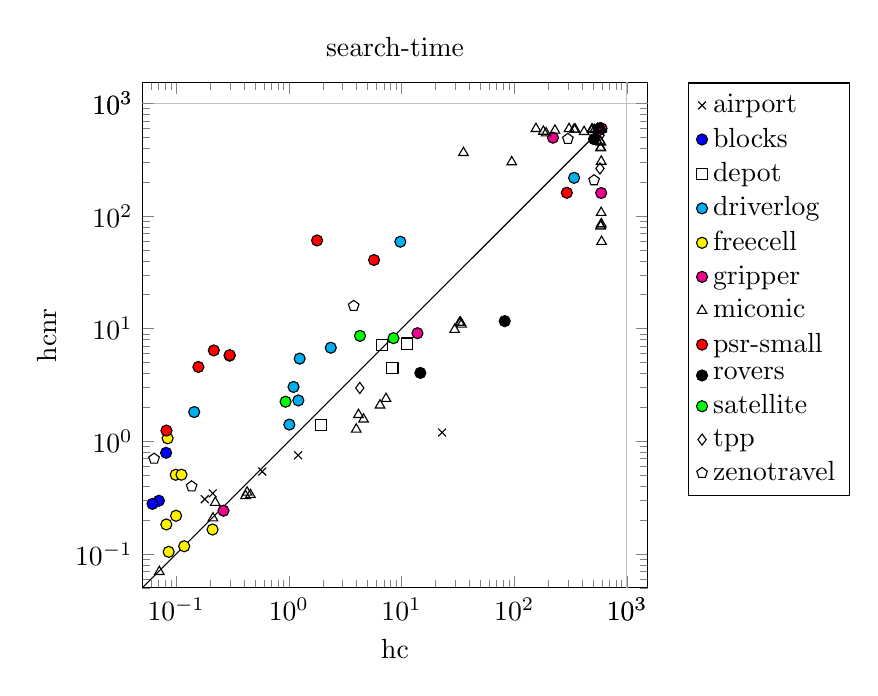
\begin{tikzpicture}
\begin{axis}[extra x tick style={grid=major}, extra x ticks=1000, extra y tick style={grid=major}, 
extra y ticks=1000, height=8cm, legend cell align=left, legend style={at={(1.4, 1)}}, title=search-time, width=8cm, xlabel=hc, xmin=0.05, xmode=log, ylabel=hcnr, ymin=0.05, ymode=log]
\addplot[color=green, mark=x, mark options={{draw=black}}, only marks] coordinates {
(0.580962, 0.539156) (22.919350, 1.197450) (1.207802, 0.751533) (0.010000, 0.010000) (0.211029, 0.344864) (0.179368, 0.306256)
};
\addlegendentry{airport}
\addplot[color=blue, mark=*, mark options={{draw=black}}, only marks] coordinates {
(0.070254, 0.296864) (0.031537, 0.132323) (0.061611, 0.278351) (0.010000, 0.015546) (0.081349, 0.790786) (0.032068, 0.459737) (0.010000, 0.022621) (0.038953, 0.506324) (0.024986, 0.185765) (0.010000, 0.019080) (0.010000, 0.010000) (0.010000, 0.045402) (0.011799, 0.083719)
};
\addlegendentry{blocks}
\addplot[color=magenta, mark=square, mark options={{draw=black}}, only marks] coordinates {
(11.217900, 7.372310) (0.010000, 0.032782) (6.757340, 7.158310) (0.010000, 0.010000) (8.306120, 4.493250) (1.943620, 1.390270)
};
\addlegendentry{depot}
\addplot[color=cyan, mark=*, mark options={{draw=black}}, only marks] coordinates {
(0.297981, 5.756450) (0.144535, 1.819230) (1.100020, 3.040280) (1.214180, 2.305950) (340.116000, 218.241000) (9.760760, 59.133700) (1.246790, 5.421790) (1.009640, 1.408210) (0.013146, 0.044778) (0.010000, 0.010000) (2.354820, 6.773570)
};
\addlegendentry{driverlog}
\addplot[color=yellow, mark=*, mark options={{draw=black}}, only marks] coordinates {
(0.099746, 0.218327) (0.210252, 0.164829) (0.042857, 0.142258) (0.013246, 0.016653) (0.117766, 0.117104) (0.099051, 0.504578) (0.083962, 1.063150) (0.010000, 0.023282) (0.037383, 0.106107) (0.141554, 0.013294) (0.081759, 0.182805) (0.111385, 0.505483) (0.025328, 0.024882) (0.085739, 0.104453)
};
\addlegendentry{freecell}
\addplot[color=magenta, mark=*, mark options={{draw=black}}, only marks] coordinates {
(0.262926, 0.241988) (220.812500, 495.988300) (596.647608, 597.565062) (569.492855, 580.212440) (0.010000, 0.010000) (13.844100, 9.110310) (591.089502, 160.080000)
};
\addlegendentry{gripper}
\addplot[color=cyan, mark=triangle, mark options={{draw=black}}, only marks] coordinates {
(339.622700, 588.378030) (0.010000, 0.011511) (549.845320, 596.864944) (590.112556, 597.189862) (7.282070, 2.391340) (0.010000, 0.012300) (0.412567, 0.327916) (584.148657, 401.133000) (6.442820, 2.091980) (0.039212, 0.046379) (3.963360, 1.277520) (590.819602, 107.059000) (586.187417, 597.268517) (306.656100, 594.349870) (95.053000, 301.677300) (34.077400, 10.919400) (181.635500, 562.785100) (0.010000, 0.012302) (35.450700, 364.431800) (594.301000, 589.966394) (592.930220, 85.041900) (585.482311, 81.044100) (0.026386, 0.042528) (570.608013, 597.167369) (347.818020, 587.793298) (155.906400, 595.750950) (32.738500, 11.323200) (596.722586, 598.978263) (0.070847, 0.069548) (191.937600, 544.281070) (577.370218, 460.882000) (496.366840, 586.208798) (0.042445, 0.049317) (592.167179, 305.104556) (0.455739, 0.335505) (29.592500, 9.804140) (0.048676, 0.049344) (4.148850, 1.722520) (585.890390, 82.624400) (0.212131, 0.208158) (586.905028, 407.188000) (577.634284, 595.238650) (588.228783, 451.849000) (517.980280, 582.901515) (0.222096, 0.285741) (488.742600, 588.815017) (596.108119, 59.254000) (229.859700, 575.452420) (4.599160, 1.569080) (0.010000, 0.010000) (33.443600, 11.359900) (0.425846, 0.352192) (417.259400, 559.410200) (0.010000, 0.012175)
};
\addlegendentry{miconic}
\addplot[color=red, mark=*, mark options={{draw=black}}, only marks] coordinates {
(0.010000, 0.011470) (0.010000, 0.032399) (293.244000, 160.887713) (0.010000, 0.012510) (0.020875, 0.200436) (0.215694, 6.411470) (0.010000, 0.019380) (0.081920, 1.245030) (0.013860, 0.108072) (0.034962, 0.448613) (0.020044, 0.175404) (0.157385, 4.569860) (0.010000, 0.044764) (0.011576, 0.024512) (0.298527, 5.820420) (0.010000, 0.010334) (0.010000, 0.058066) (1.779940, 60.661200) (0.010000, 0.020175) (0.030218, 0.282279) (0.014752, 0.078198) (0.010000, 0.010393) (0.010000, 0.031036) (0.010850, 0.076801) (0.010000, 0.015075) (0.016773, 0.031202) (0.022007, 0.111476) (0.010000, 0.010273) (0.010000, 0.010000) (5.700890, 40.694000)
};
\addlegendentry{psr-small}
\addplot[color=black, mark=*, mark options={{draw=black}}, only marks] coordinates {
(14.684900, 4.047890) (82.362900, 11.664700) (511.206762, 481.269259) (0.010000, 0.010000)
};
\addlegendentry{rovers}
\addplot[color=green, mark=*, mark options={{draw=black}}, only marks] coordinates {
(8.485640, 8.230840) (0.016291, 0.046241) (0.935294, 2.246410) (0.010000, 0.010000) (0.010000, 0.027242) (4.278860, 8.627940)
};
\addlegendentry{satellite}
\addplot[color=blue, mark=diamond, mark options={{draw=black}}, only marks] coordinates {
(578.425608, 519.404647) (4.261390, 2.976200) (0.033617, 0.096048) (576.817000, 264.094000) (0.010000, 0.010000)
};
\addlegendentry{tpp}
\addplot[color=red, mark=pentagon, mark options={{draw=black}}, only marks] coordinates {
(511.621367, 207.755000) (0.018711, 0.085917) (553.269035, 596.441548) (0.010000, 0.020608) (0.063638, 0.701225) (3.762470, 15.939800) (0.010000, 0.010000) (0.010000, 0.016045) (0.010000, 0.011999) (0.137054, 0.398511) (299.509103, 483.854610)
};
\addlegendentry{zenotravel}
\addplot[color=black] coordinates {(0.050000, 0.050000) (598, 598)};
\end{axis}
\end{tikzpicture}
\\
        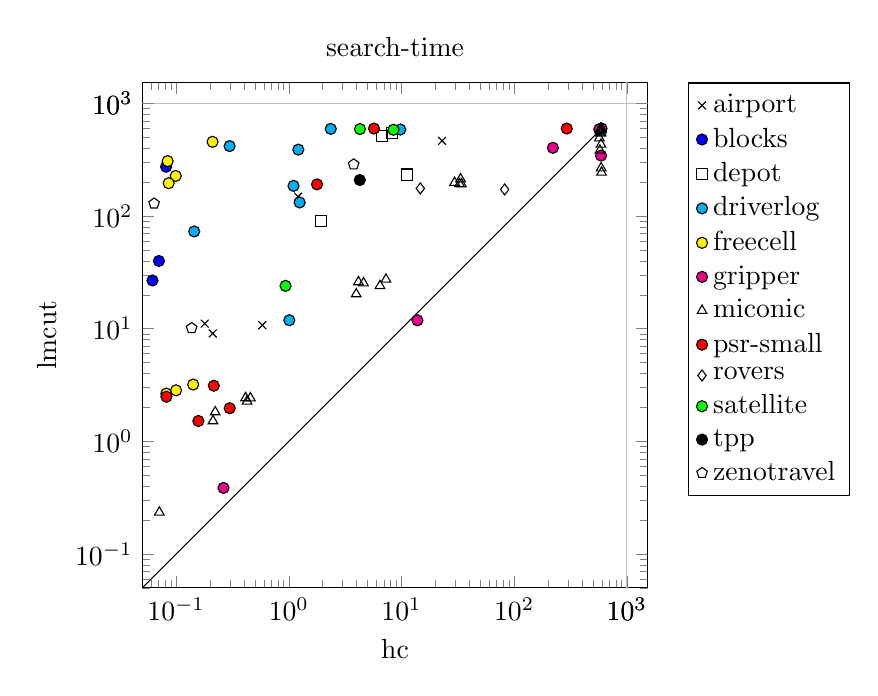
\begin{tikzpicture}
\begin{axis}[extra x tick style={grid=major}, extra x ticks=1000, extra y tick style={grid=major}, 
extra y ticks=1000, height=8.00cm, legend cell align=left, legend style={at={(1.4, 1)}}, title=search-time, width=8.00cm, xlabel=hc, xmin=0.05, xmode=log, ylabel=lmcut, ymin=0.05, ymode=log]
\addplot[color=green, mark=x, mark options={{draw=black}}, only marks] coordinates {
(0.010000, 0.145019) (0.179368, 11.087800) (0.010000, 0.148471) (22.919350, 465.248041) (0.010000, 0.138836) (1.207802, 148.594000) (0.580962, 10.739300) (0.010000, 0.010000) (0.010000, 0.144218) (0.211029, 9.069710)
};
\addlegendentry{airport}
\addplot[color=blue, mark=*, mark options={{draw=black}}, only marks] coordinates {
(0.010000, 0.241287) (0.081349, 273.943000) (0.032068, 25.498900) (0.024986, 17.856400) (0.010000, 0.013831) (0.010000, 0.011050) (0.010000, 0.014994) (0.070254, 39.917200) (0.011799, 1.396270) (0.031537, 2.845540) (0.038953, 56.848500) (0.010000, 0.010000) (0.061611, 26.801200) (0.010000, 0.084920) (0.010000, 0.143467) (0.010000, 0.053145)
};
\addlegendentry{blocks}
\addplot[color=magenta, mark=square, mark options={{draw=black}}, only marks] coordinates {
(8.306120, 546.413867) (0.010000, 0.454776) (0.010000, 0.010000) (11.217900, 233.682000) (6.757340, 513.742809) (1.943620, 90.322400)
};
\addlegendentry{depot}
\addplot[color=cyan, mark=*, mark options={{draw=black}}, only marks] coordinates {
(2.354820, 594.273762) (1.100020, 185.435000) (1.214180, 388.772000) (9.760760, 585.985461) (0.013146, 0.355551) (0.297981, 417.908000) (0.010000, 0.010000) (1.009640, 11.880900) (0.144535, 73.016200) (1.246790, 132.045000)
};
\addlegendentry{driverlog}
\addplot[color=yellow, mark=*, mark options={{draw=black}}, only marks] coordinates {
(0.099051, 227.105000) (0.083962, 307.362000) (0.210252, 455.826000) (0.042857, 2.234200) (0.010000, 0.197040) (0.099746, 2.836240) (0.037383, 2.066460) (0.085739, 195.725000) (0.013246, 14.349400) (0.081759, 2.653950) (0.025328, 255.793000) (0.141554, 3.192820)
};
\addlegendentry{freecell}
\addplot[color=magenta, mark=*, mark options={{draw=black}}, only marks] coordinates {
(591.089502, 344.121000) (0.262926, 0.385840) (596.647608, 599.519963) (569.492855, 589.232378) (13.844100, 11.876000) (220.812500, 403.291000) (0.010000, 0.014257)
};
\addlegendentry{gripper}
\addplot[color=cyan, mark=triangle, mark options={{draw=black}}, only marks] coordinates {
(7.282070, 27.391700) (590.112556, 432.887000) (0.212131, 1.517590) (0.425846, 2.264950) (32.738500, 192.940000) (0.222096, 1.820830) (584.148657, 587.696141) (0.026386, 0.169860) (577.370218, 579.753396) (0.048676, 0.217090) (596.722586, 243.971000) (586.187417, 543.923243) (0.455739, 2.420320) (585.890390, 587.271962) (0.039212, 0.219873) (592.930220, 585.958915) (4.148850, 26.007800) (570.608013, 491.997000) (0.010000, 0.030098) (0.010000, 0.028190) (0.042445, 0.204913) (585.482311, 597.641841) (4.599160, 25.405300) (6.442820, 24.030000) (590.819602, 595.781666) (0.010000, 0.027890) (592.167179, 266.793000) (33.443600, 213.065000) (596.108119, 593.064799) (0.010000, 0.029482) (0.070847, 0.234214) (34.077400, 192.393000) (0.412567, 2.426510) (3.963360, 20.321900) (586.905028, 579.938124) (29.592500, 197.966000) (588.228783, 555.366355) (0.010000, 0.010000) (0.010000, 0.028766) (577.634284, 383.340000)
};
\addlegendentry{miconic}
\addplot[color=red, mark=*, mark options={{draw=black}}, only marks] coordinates {
(0.215694, 3.116640) (0.022007, 0.131474) (0.157385, 1.515700) (0.010000, 0.063653) (0.010000, 0.015288) (5.700890, 597.876933) (0.010000, 0.439747) (0.034962, 0.159061) (0.010000, 0.014646) (0.020044, 0.123132) (0.014752, 0.084136) (0.010000, 0.013838) (0.010000, 0.010526) (293.244000, 598.462153) (0.010000, 0.057526) (0.011576, 0.033149) (0.020875, 0.073845) (0.010000, 0.035914) (0.016773, 0.010000) (0.081920, 2.488950) (1.779940, 191.082000) (0.010000, 0.014621) (0.010850, 0.058979) (0.010000, 0.032497) (0.298527, 1.967380) (0.030218, 0.126164) (0.010000, 0.010000) (0.013860, 0.053829) (0.010000, 0.043889)
};
\addlegendentry{psr-small}
\addplot[color=blue, mark=diamond, mark options={{draw=black}}, only marks] coordinates {
(14.684900, 175.966000) (0.010000, 0.012330) (82.362900, 172.156000) (0.010000, 0.010000)
};
\addlegendentry{rovers}
\addplot[color=green, mark=*, mark options={{draw=black}}, only marks] coordinates {
(0.010000, 0.037315) (0.935294, 24.005000) (8.485640, 583.323190) (0.016291, 0.290613) (4.278860, 591.951665) (0.010000, 0.010000)
};
\addlegendentry{satellite}
\addplot[color=black, mark=*, mark options={{draw=black}}, only marks] coordinates {
(0.010000, 0.021228) (0.010000, 0.010000) (0.033617, 0.729151) (4.261390, 208.745000)
};
\addlegendentry{tpp}
\addplot[color=red, mark=pentagon, mark options={{draw=black}}, only marks] coordinates {
(0.137054, 10.125700) (0.010000, 0.010000) (0.063638, 129.227000) (0.010000, 0.089784) (0.010000, 0.426249) (3.762470, 287.667000) (0.010000, 0.149214) (0.018711, 4.364840)
};
\addlegendentry{zenotravel}
\addplot[color=black] coordinates {(0.050000, 0.050000) (599, 599)};
\end{axis}
\end{tikzpicture}
\\
        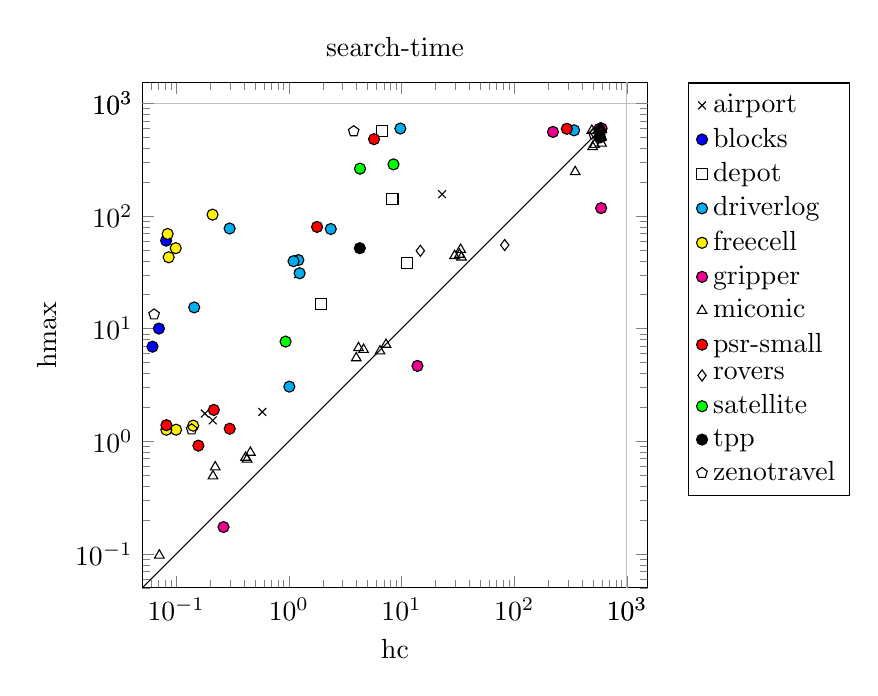
\begin{tikzpicture}
\begin{axis}[extra x tick style={grid=major}, extra x ticks=1000, extra y tick style={grid=major}, 
extra y ticks=1000, height=8.00cm, legend cell align=left, legend style={at={(1.4, 1)}}, title=search-time, width=8.00cm, xlabel=hc, xmin=0.05, xmode=log, ylabel=hmax, ymin=0.05, ymode=log]
\addplot[color=green, mark=x, mark options={{draw=black}}, only marks] coordinates {
(0.211029, 1.535550) (0.179368, 1.763850) (22.919350, 156.197000) (1.207802, 30.523000) (0.010000, 0.035344) (0.010000, 0.035362) (0.010000, 0.031154) (0.010000, 0.037047) (0.010000, 0.010000) (0.580962, 1.822400)
};
\addlegendentry{airport}
\addplot[color=blue, mark=*, mark options={{draw=black}}, only marks] coordinates {
(0.032068, 5.732710) (0.070254, 10.017100) (0.010000, 0.047037) (0.010000, 0.012368) (0.061611, 6.917790) (0.010000, 0.012243) (0.038953, 12.781400) (0.010000, 0.113656) (0.031537, 0.862602) (0.024986, 4.632420) (0.010000, 0.010000) (0.011799, 0.439723) (0.010000, 0.064324) (0.081349, 60.444000) (0.010000, 0.033449)
};
\addlegendentry{blocks}
\addplot[color=magenta, mark=square, mark options={{draw=black}}, only marks] coordinates {
(0.010000, 0.127047) (1.943620, 16.555100) (11.217900, 38.239000) (8.306120, 140.910000) (0.010000, 0.010000) (6.757340, 565.255782)
};
\addlegendentry{depot}
\addplot[color=cyan, mark=*, mark options={{draw=black}}, only marks] coordinates {
(0.297981, 77.459500) (9.760760, 597.749223) (0.013146, 0.115082) (2.354820, 76.663600) (1.009640, 3.057640) (0.144535, 15.437500) (1.246790, 31.041800) (1.214180, 40.615900) (0.010000, 0.010000) (1.100020, 39.711100) (340.116000, 575.892081)
};
\addlegendentry{driverlog}
\addplot[color=yellow, mark=*, mark options={{draw=black}}, only marks] coordinates {
(0.025328, 59.011600) (0.210252, 102.793000) (0.010000, 0.124281) (0.099746, 1.267980) (0.083962, 69.265900) (0.141554, 1.376880) (0.042857, 1.066010) (0.037383, 1.096480) (0.081759, 1.266610) (0.013246, 3.938400) (0.099051, 51.804200) (0.085739, 43.038000)
};
\addlegendentry{freecell}
\addplot[color=magenta, mark=*, mark options={{draw=black}}, only marks] coordinates {
(13.844100, 4.669780) (596.647608, 598.667659) (591.089502, 117.455000) (0.262926, 0.173503) (569.492855, 593.108070) (0.010000, 0.010000) (220.812500, 557.649400)
};
\addlegendentry{gripper}
\addplot[color=cyan, mark=triangle, mark options={{draw=black}}, only marks] coordinates {
(0.425846, 0.692233) (4.599160, 6.511650) (588.228783, 591.122512) (0.212131, 0.491115) (3.963360, 5.488040) (6.442820, 6.315310) (517.980280, 429.754000) (0.048676, 0.089155) (0.455739, 0.795860) (577.634284, 561.149300) (347.818020, 246.674000) (0.222096, 0.591140) (0.070847, 0.097298) (577.370218, 598.055292) (34.077400, 43.061700) (29.592500, 44.360300) (4.148850, 6.747270) (592.167179, 595.122680) (596.722586, 585.635170) (592.930220, 499.164000) (586.905028, 594.884152) (590.112556, 578.235044) (596.108119, 441.372000) (549.845320, 569.778350) (0.010000, 0.014717) (33.443600, 50.381600) (0.412567, 0.717870) (585.482311, 493.436000) (586.187417, 592.331096) (0.039212, 0.088437) (594.301000, 509.525200) (0.010000, 0.015111) (488.742600, 574.346900) (570.608013, 589.738525) (584.148657, 595.027433) (0.026386, 0.071008) (585.890390, 494.009000) (496.366840, 410.867000) (0.010000, 0.014640) (7.282070, 7.229640) (0.010000, 0.015968) (590.819602, 595.820423) (0.042445, 0.083550) (0.010000, 0.010000) (32.738500, 45.512700) (0.010000, 0.014809)
};
\addlegendentry{miconic}
\addplot[color=red, mark=*, mark options={{draw=black}}, only marks] coordinates {
(0.022007, 0.186275) (0.010000, 0.013324) (0.010850, 0.048356) (0.010000, 0.046423) (0.010000, 0.062220) (0.013860, 0.058309) (0.010000, 0.021642) (0.020044, 0.096882) (0.010000, 0.045396) (0.010000, 0.012186) (5.700890, 480.711000) (1.779940, 80.007200) (0.215694, 1.899360) (0.030218, 0.140215) (0.020875, 0.055608) (0.010000, 0.017516) (0.034962, 0.155076) (0.011576, 0.011249) (0.010000, 0.012182) (0.010000, 0.045889) (0.010000, 0.010726) (0.010000, 0.013610) (0.016773, 0.010000) (0.010000, 0.020060) (0.010000, 0.018839) (0.014752, 0.110608) (293.244000, 594.306057) (0.081920, 1.389790) (0.157385, 0.915276) (0.298527, 1.293440) (0.010000, 0.010000) (0.010000, 0.038902)
};
\addlegendentry{psr-small}
\addplot[color=blue, mark=diamond, mark options={{draw=black}}, only marks] coordinates {
(82.362900, 55.198900) (511.206762, 551.957520) (14.684900, 49.125200) (0.010000, 0.010000)
};
\addlegendentry{rovers}
\addplot[color=green, mark=*, mark options={{draw=black}}, only marks] coordinates {
(0.016291, 0.140580) (0.010000, 0.021659) (0.935294, 7.679300) (4.278860, 263.238000) (0.010000, 0.010000) (8.485640, 287.232000)
};
\addlegendentry{satellite}
\addplot[color=black, mark=*, mark options={{draw=black}}, only marks] coordinates {
(576.817000, 498.468930) (0.033617, 0.280404) (4.261390, 51.802300) (0.010000, 0.010000) (0.010000, 0.013405)
};
\addlegendentry{tpp}
\addplot[color=red, mark=pentagon, mark options={{draw=black}}, only marks] coordinates {
(0.010000, 0.066958) (3.762470, 565.487054) (511.621367, 529.978709) (0.063638, 13.368700) (0.137054, 1.276830) (0.010000, 0.036161) (0.010000, 0.010000) (0.010000, 0.046869) (0.018711, 0.643291)
};
\addlegendentry{zenotravel}
\addplot[color=black] coordinates {(0.050000, 0.050000) (598, 598)};
\end{axis}
\end{tikzpicture}
\\
        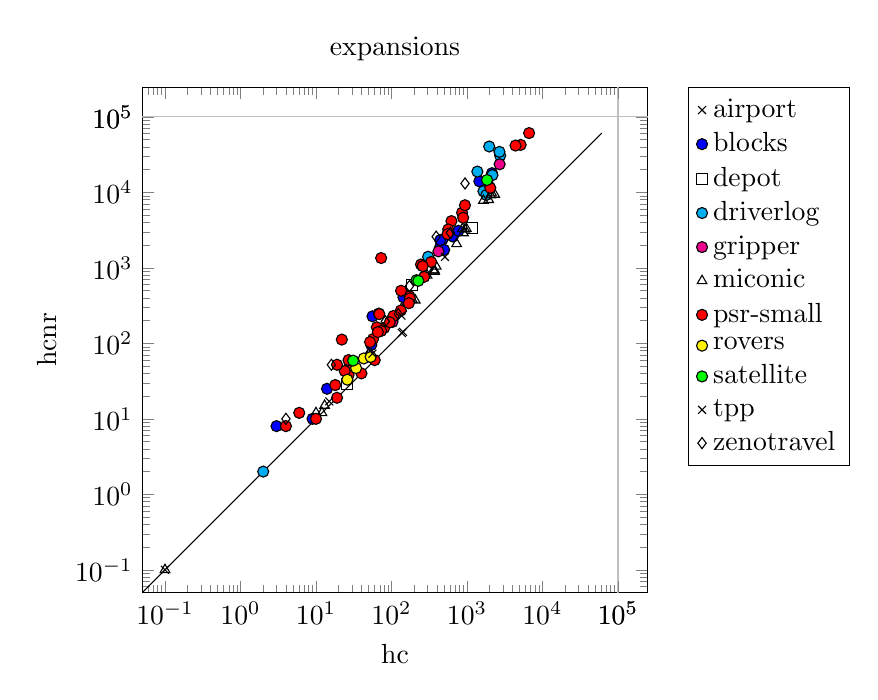
\begin{tikzpicture}
\begin{axis}[extra x tick style={grid=major}, extra x ticks=100000, extra y tick style={grid=major}, 
extra y ticks=100000, height=8.00cm, legend cell align=left, legend style={at={(1.4, 1)}}, title=expansions, width=8.00cm, xlabel=hc, xmin=0.05, xmode=log, ylabel=hcnr, ymin=0.05, ymode=log]
\addplot[color=red, mark=x, mark options={{draw=black}}, only marks] coordinates {
(0.100000, 0.100000) (137, 137) (142, 142)
};
\addlegendentry{airport}
\addplot[color=blue, mark=*, mark options={{draw=black}}, only marks] coordinates {
(100, 202) (1875, 13298) (2144, 17941) (439, 1855) (651, 2599) (3, 8) (14, 25) (499, 1732) (144, 407) (56, 228) (9, 10) (106, 219) (1458, 14012) (474, 2375) (70, 149) (54, 95) (770, 3093) (442, 2329)
};
\addlegendentry{blocks}
\addplot[color=cyan, mark=square, mark options={{draw=black}}, only marks] coordinates {
(1165, 3337) (26, 29) (186, 594)
};
\addlegendentry{depot}
\addplot[color=cyan, mark=*, mark options={{draw=black}}, only marks] coordinates {
(2176, 16918) (1652, 10340) (1805, 9221) (306, 1402) (1971, 40492) (2, 2) (2754, 30702) (1373, 18842) (2695, 34370)
};
\addlegendentry{driverlog}
\addplot[color=magenta, mark=*, mark options={{draw=black}}, only marks] coordinates {
(103, 192) (2708, 23542) (419, 1653)
};
\addlegendentry{gripper}
\addplot[color=blue, mark=triangle, mark options={{draw=black}}, only marks] coordinates {
(981, 3311) (1651, 7795) (188, 381) (2121, 9781) (12, 12) (371, 930) (730, 2078) (52, 77) (372, 890) (1940, 7993) (48, 63) (359, 929) (10, 12) (937, 3229) (51, 66) (164, 345) (0.100000, 0.100000) (47, 66) (46, 62) (13, 15) (2333, 9377) (296, 797) (391, 1046) (136, 290) (207, 372) (901, 2892) (2060, 9235) (867, 3283) (164, 351)
};
\addlegendentry{miconic}
\addplot[color=red, mark=*, mark options={{draw=black}}, only marks] coordinates {
(271, 760) (19, 19) (4, 8) (28, 55) (106, 230) (22, 112) (173, 421) (246, 1106) (27, 38) (5143, 42522) (68, 248) (27, 60) (861, 5382) (891, 4609) (60, 60) (80, 160) (64, 163) (6652, 60966) (24, 43) (57, 114) (73, 1348) (175, 395) (69, 244) (623, 4157) (18, 28) (52, 104) (73, 146) (6, 12) (2036, 11460) (95, 190) (134, 497) (564, 3227) (133, 272) (10, 10) (552, 2794) (335, 1194) (66, 141) (40, 40) (259, 1053) (941, 6750) (4401, 41680) (19, 52) (170, 340)
};
\addlegendentry{psr-small}
\addplot[color=yellow, mark=*, mark options={{draw=black}}, only marks] coordinates {
(34, 47) (43, 63) (53, 66) (26, 33)
};
\addlegendentry{rovers}
\addplot[color=green, mark=*, mark options={{draw=black}}, only marks] coordinates {
(214, 686) (227, 673) (1844, 14576) (31, 59)
};
\addlegendentry{satellite}
\addplot[color=green, mark=x, mark options={{draw=black}}, only marks] coordinates {
(56, 73) (136, 233) (511, 1394) (15, 17)
};
\addlegendentry{tpp}
\addplot[color=black, mark=diamond, mark options={{draw=black}}, only marks] coordinates {
(942, 13116) (123, 244) (4, 10) (173, 573) (16, 52) (602, 2919) (391, 2589) (83, 195)
};
\addlegendentry{zenotravel}
\addplot[color=black] coordinates {(0.050000, 0.050000) (60966, 60966)};
\end{axis}
\end{tikzpicture}
\\
        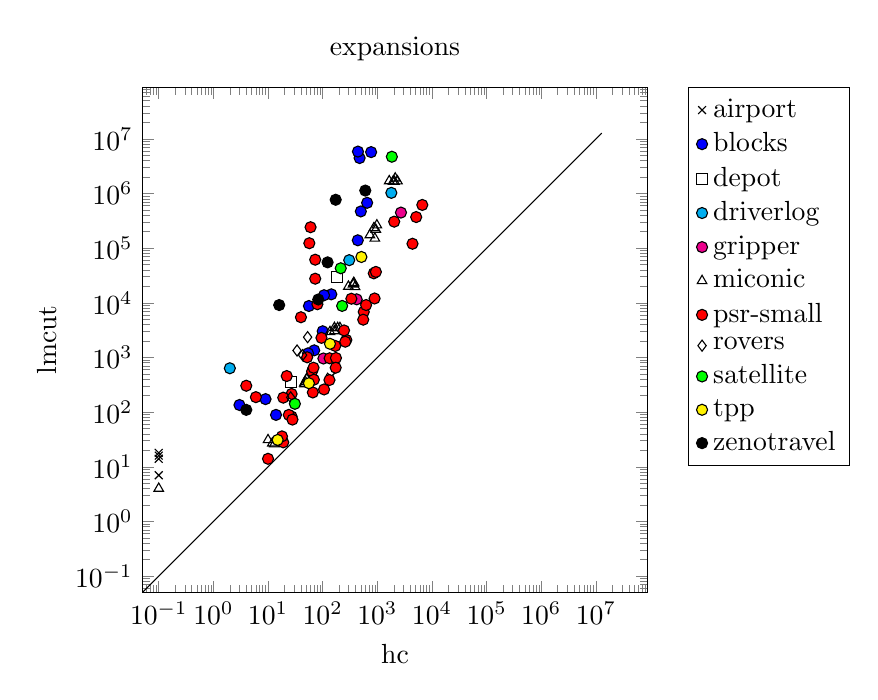
\begin{tikzpicture}
\begin{axis}[extra x tick style={grid=major}, extra x ticks=100000000, extra y tick style={grid=major}, extra y ticks=100000000, height=8.00cm, 
legend cell align=left, legend style={at={(1.4, 1)}}, title=expansions, width=8.00cm, xlabel=hc, xmin=0.05, xmode=log, ylabel=lmcut, ymin=0.05, ymode=log]
\addplot[color=red, mark=x, mark options={{draw=black}}, only marks] coordinates {
(142, 444) (0.100000, 14) (0.100000, 18) (0.100000, 7) (0.100000, 16) (137, 421)
};
\addlegendentry{airport}
\addplot[color=blue, mark=*, mark options={{draw=black}}, only marks] coordinates {
(9, 173) (474, 4460545) (100, 3018) (439, 139356) (14, 89) (144, 14312) (442, 5854588) (106, 13778) (56, 8750) (651, 676067) (770, 5723779) (3, 135) (70, 1350) (54, 1191) (499, 470462)
};
\addlegendentry{blocks}
\addplot[color=cyan, mark=square, mark options={{draw=black}}, only marks] coordinates {
(186, 30045) (26, 362)
};
\addlegendentry{depot}
\addplot[color=cyan, mark=*, mark options={{draw=black}}, only marks] coordinates {
(306, 60344) (1805, 1028572) (2, 635)
};
\addlegendentry{driverlog}
\addplot[color=magenta, mark=*, mark options={{draw=black}}, only marks] coordinates {
(103, 958) (419, 11586) (2708, 448198)
};
\addlegendentry{gripper}
\addplot[color=blue, mark=triangle, mark options={{draw=black}}, only marks] coordinates {
(2121, 1903853) (372, 22499) (48, 361) (13, 26) (52, 424) (391, 19586) (1940, 1650838) (12, 27) (730, 174147) (1651, 1697048) (51, 400) (2333, 1690274) (47, 327) (901, 151003) (359, 21853) (10, 31) (188, 3492) (46, 336) (371, 23396) (981, 263639) (207, 3488) (296, 19955) (0.100000, 4) (164, 3060) (867, 234915) (136, 2947) (937, 219412) (164, 3501) (2060, 1656771)
};
\addlegendentry{miconic}
\addplot[color=red, mark=*, mark options={{draw=black}}, only marks] coordinates {
(271, 2092) (27, 215) (861, 34633) (64, 557) (27, 83) (40, 5446) (80, 9432) (564, 6833) (73, 27640) (73, 61548) (6652, 618078) (259, 1944) (106, 260) (4401, 120468) (4, 304) (24, 89) (10, 14) (19, 28) (52, 1008) (623, 9112) (28, 73) (57, 123268) (95, 2286) (891, 12005) (552, 4917) (22, 457) (134, 967) (69, 392) (133, 387) (68, 649) (60, 241899) (335, 11892) (6, 188) (5143, 370920) (18, 36) (19, 184) (170, 1626) (175, 979) (66, 229) (941, 36799) (173, 650) (246, 3125) (2036, 305520)
};
\addlegendentry{psr-small}
\addplot[color=green, mark=diamond, mark options={{draw=black}}, only marks] coordinates {
(34, 1343) (43, 1106) (53, 2354) (26, 186)
};
\addlegendentry{rovers}
\addplot[color=green, mark=*, mark options={{draw=black}}, only marks] coordinates {
(214, 42892) (31, 142) (227, 8777) (1844, 4711577)
};
\addlegendentry{satellite}
\addplot[color=yellow, mark=*, mark options={{draw=black}}, only marks] coordinates {
(511, 69014) (136, 1779) (15, 31) (56, 338)
};
\addlegendentry{tpp}
\addplot[color=black, mark=*, mark options={{draw=black}}, only marks] coordinates {
(602, 1133103) (16, 9104) (4, 110) (123, 55014) (83, 11510) (173, 769022)
};
\addlegendentry{zenotravel}
\addplot[color=black] coordinates {(0.050000, 0.050000) (12763448, 12763448)};
\end{axis}
\end{tikzpicture}
\\
        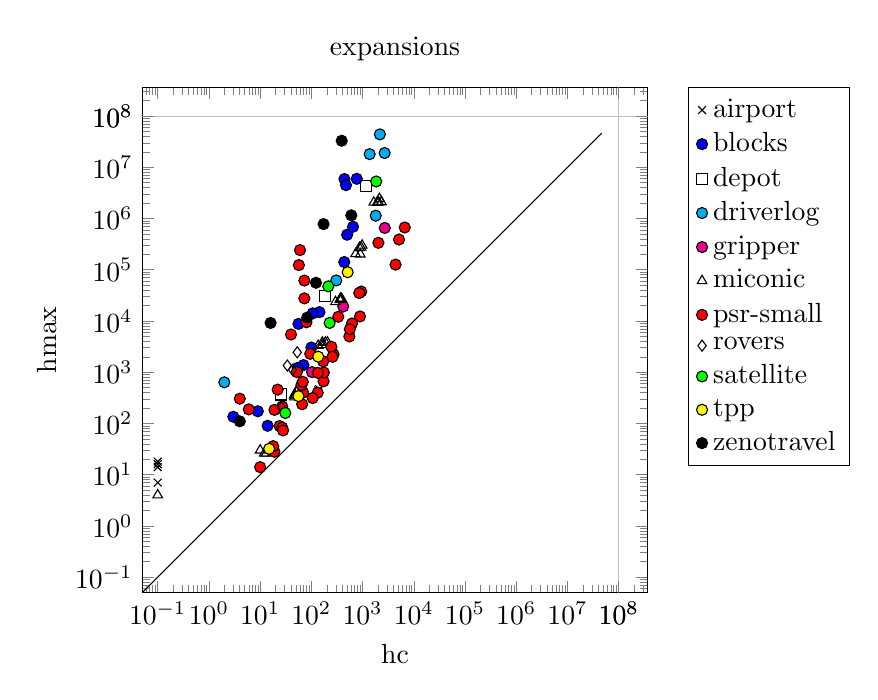
\begin{tikzpicture}
\begin{axis}[extra x tick style={grid=major}, extra x ticks=100000000, extra y tick style={grid=major}, extra y ticks=100000000, height=8.00cm,
 legend cell align=left, legend style={at={(1.4, 1)}}, title=expansions, width=8.00cm, xlabel=hc, xmin=0.05, xmode=log, ylabel=hmax, ymin=0.05, ymode=log]
\addplot[color=red, mark=x, mark options={{draw=black}}, only marks] coordinates {
(142, 464) (0.100000, 14) (0.100000, 18) (0.100000, 7) (0.100000, 16) (137, 441)
};
\addlegendentry{airport}
\addplot[color=blue, mark=*, mark options={{draw=black}}, only marks] coordinates {
(144, 14897) (9, 173) (442, 5894179) (70, 1376) (499, 483086) (56, 8783) (439, 141443) (100, 3031) (14, 90) (3, 135) (474, 4487213) (54, 1215) (651, 691186) (106, 14089) (770, 5968890)
};
\addlegendentry{blocks}
\addplot[color=cyan, mark=square, mark options={{draw=black}}, only marks] coordinates {
(186, 30239) (1165, 4348281) (26, 368)
};
\addlegendentry{depot}
\addplot[color=cyan, mark=*, mark options={{draw=black}}, only marks] coordinates {
(306, 61958) (1373, 18078718) (2695, 19007847) (1805, 1136659) (2, 635) (2176, 43967863)
};
\addlegendentry{driverlog}
\addplot[color=magenta, mark=*, mark options={{draw=black}}, only marks] coordinates {
(419, 19191) (103, 1006) (2708, 655342)
};
\addlegendentry{gripper}
\addplot[color=blue, mark=triangle, mark options={{draw=black}}, only marks] coordinates {
(51, 424) (372, 27235) (207, 3838) (13, 26) (1940, 2054791) (2333, 2104717) (48, 359) (10, 30) (188, 3838) (164, 3428) (46, 353) (47, 327) (730, 203857) (0.100000, 4) (981, 299347) (901, 201439) (937, 273423) (867, 269792) (136, 3311) (391, 27181) (371, 27525) (1651, 2066634) (296, 23696) (2121, 2441914) (2060, 2086171) (12, 26) (164, 3838) (52, 422) (359, 25847)
};
\addlegendentry{miconic}
\addplot[color=red, mark=*, mark options={{draw=black}}, only marks] coordinates {
(27, 215) (552, 4995) (133, 397) (335, 12092) (66, 237) (623, 8950) (40, 5446) (80, 9432) (73, 27640) (73, 61548) (271, 2230) (69, 400) (106, 313) (4, 304) (24, 89) (5143, 389358) (10, 14) (52, 1008) (19, 28) (57, 123268) (173, 665) (95, 2286) (891, 12261) (4401, 126004) (27, 83) (64, 561) (22, 457) (564, 6921) (6652, 668998) (175, 987) (68, 649) (60, 241899) (246, 3131) (6, 188) (134, 970) (28, 73) (18, 36) (2036, 335904) (19, 184) (170, 1626) (259, 2000) (941, 37611) (861, 35149)
};
\addlegendentry{psr-small}
\addplot[color=green, mark=diamond, mark options={{draw=black}}, only marks] coordinates {
(26, 207) (34, 1350) (53, 2442) (43, 1113)
};
\addlegendentry{rovers}
\addplot[color=green, mark=*, mark options={{draw=black}}, only marks] coordinates {
(227, 9176) (214, 47435) (1844, 5287951) (31, 160)
};
\addlegendentry{satellite}
\addplot[color=yellow, mark=*, mark options={{draw=black}}, only marks] coordinates {
(511, 89604) (56, 341) (15, 32) (136, 2013)
};
\addlegendentry{tpp}
\addplot[color=black, mark=*, mark options={{draw=black}}, only marks] coordinates {
(4, 110) (16, 9148) (123, 55748) (602, 1155505) (83, 11658) (391, 33028328) (173, 778708)
};
\addlegendentry{zenotravel}
\addplot[color=black] coordinates {(0.050000, 0.050000) (46590097, 46590097)};
\end{axis}
\end{tikzpicture}

    \end{center}
   

    \subsubsection*{Cost Bound 0.5}

    \begin{center}

        \begin{tabular}{l|r|r|r|r}
            Finished PPD1 & hc & hcnr & hmax & lmcut \\\hline
            airport (19) & 12 & 12 & \textbf{16} & 15\\\hline
            blocks (18) & 18 & 18 & 18 & 18 \\\hline
            depot (6) & \textbf{6} & \textbf{6} & 5 & 4 \\\hline
            driverlog (11) & \textbf{11} & \textbf{11} & 9 & 8 \\\hline
            freecell (55) & 6 & 7 & \textbf{15} & 14 \\\hline
            gripper (8) & 3 & \textbf{4} & \textbf{4} & \textbf{4} \\\hline
            miconic (69) & 39 & \textbf{48} & 43 & 39 \\\hline
            PSR (49) & \textbf{49} & 48 & 48 & 47 \\\hline
            rovers (7) & 6 & 6 & 6 & 6 \\\hline
            satellite (6) & \textbf{6} & \textbf{6} & \textbf{6} & 4 \\\hline
            tpp (10) & \textbf{6} & \textbf{6} & 5 & 5 \\\hline
            zenotravel (11) & 8 & \textbf{9} & 7 & 7 \\\hline\hline
            sum (269) & 170 & 181 & \textbf{182} & 171 \\
        \end{tabular}

        \scriptsize
        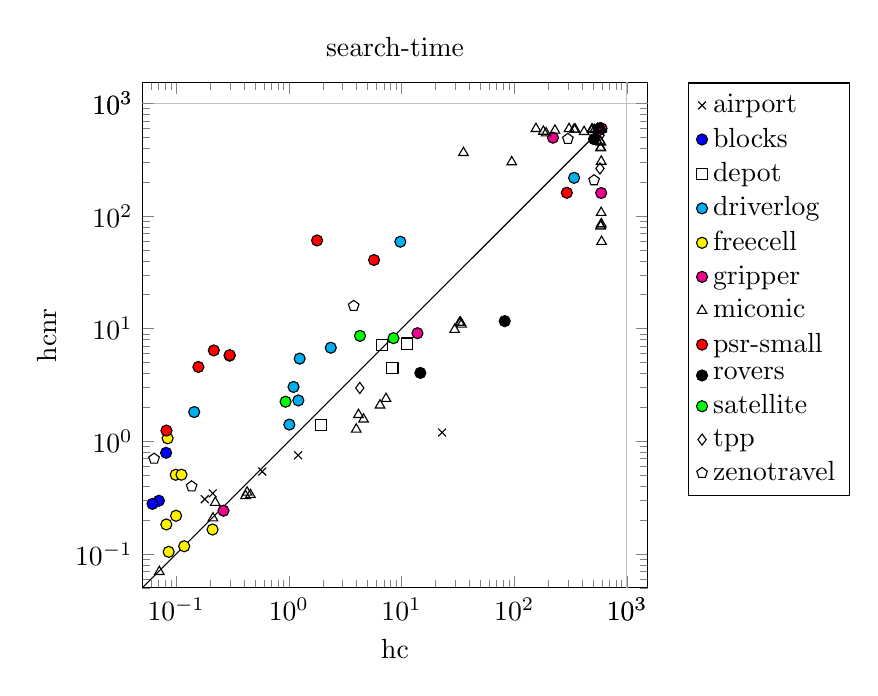
\begin{tikzpicture}
\begin{axis}[extra x tick style={grid=major}, extra x ticks=1000, extra y tick style={grid=major}, 
extra y ticks=1000, height=8cm, legend cell align=left, legend style={at={(1.4, 1)}}, title=search-time, width=8cm, xlabel=hc, xmin=0.05, xmode=log, ylabel=hcnr, ymin=0.05, ymode=log]
\addplot[color=green, mark=x, mark options={{draw=black}}, only marks] coordinates {
(0.580962, 0.539156) (22.919350, 1.197450) (1.207802, 0.751533) (0.010000, 0.010000) (0.211029, 0.344864) (0.179368, 0.306256)
};
\addlegendentry{airport}
\addplot[color=blue, mark=*, mark options={{draw=black}}, only marks] coordinates {
(0.070254, 0.296864) (0.031537, 0.132323) (0.061611, 0.278351) (0.010000, 0.015546) (0.081349, 0.790786) (0.032068, 0.459737) (0.010000, 0.022621) (0.038953, 0.506324) (0.024986, 0.185765) (0.010000, 0.019080) (0.010000, 0.010000) (0.010000, 0.045402) (0.011799, 0.083719)
};
\addlegendentry{blocks}
\addplot[color=magenta, mark=square, mark options={{draw=black}}, only marks] coordinates {
(11.217900, 7.372310) (0.010000, 0.032782) (6.757340, 7.158310) (0.010000, 0.010000) (8.306120, 4.493250) (1.943620, 1.390270)
};
\addlegendentry{depot}
\addplot[color=cyan, mark=*, mark options={{draw=black}}, only marks] coordinates {
(0.297981, 5.756450) (0.144535, 1.819230) (1.100020, 3.040280) (1.214180, 2.305950) (340.116000, 218.241000) (9.760760, 59.133700) (1.246790, 5.421790) (1.009640, 1.408210) (0.013146, 0.044778) (0.010000, 0.010000) (2.354820, 6.773570)
};
\addlegendentry{driverlog}
\addplot[color=yellow, mark=*, mark options={{draw=black}}, only marks] coordinates {
(0.099746, 0.218327) (0.210252, 0.164829) (0.042857, 0.142258) (0.013246, 0.016653) (0.117766, 0.117104) (0.099051, 0.504578) (0.083962, 1.063150) (0.010000, 0.023282) (0.037383, 0.106107) (0.141554, 0.013294) (0.081759, 0.182805) (0.111385, 0.505483) (0.025328, 0.024882) (0.085739, 0.104453)
};
\addlegendentry{freecell}
\addplot[color=magenta, mark=*, mark options={{draw=black}}, only marks] coordinates {
(0.262926, 0.241988) (220.812500, 495.988300) (596.647608, 597.565062) (569.492855, 580.212440) (0.010000, 0.010000) (13.844100, 9.110310) (591.089502, 160.080000)
};
\addlegendentry{gripper}
\addplot[color=cyan, mark=triangle, mark options={{draw=black}}, only marks] coordinates {
(339.622700, 588.378030) (0.010000, 0.011511) (549.845320, 596.864944) (590.112556, 597.189862) (7.282070, 2.391340) (0.010000, 0.012300) (0.412567, 0.327916) (584.148657, 401.133000) (6.442820, 2.091980) (0.039212, 0.046379) (3.963360, 1.277520) (590.819602, 107.059000) (586.187417, 597.268517) (306.656100, 594.349870) (95.053000, 301.677300) (34.077400, 10.919400) (181.635500, 562.785100) (0.010000, 0.012302) (35.450700, 364.431800) (594.301000, 589.966394) (592.930220, 85.041900) (585.482311, 81.044100) (0.026386, 0.042528) (570.608013, 597.167369) (347.818020, 587.793298) (155.906400, 595.750950) (32.738500, 11.323200) (596.722586, 598.978263) (0.070847, 0.069548) (191.937600, 544.281070) (577.370218, 460.882000) (496.366840, 586.208798) (0.042445, 0.049317) (592.167179, 305.104556) (0.455739, 0.335505) (29.592500, 9.804140) (0.048676, 0.049344) (4.148850, 1.722520) (585.890390, 82.624400) (0.212131, 0.208158) (586.905028, 407.188000) (577.634284, 595.238650) (588.228783, 451.849000) (517.980280, 582.901515) (0.222096, 0.285741) (488.742600, 588.815017) (596.108119, 59.254000) (229.859700, 575.452420) (4.599160, 1.569080) (0.010000, 0.010000) (33.443600, 11.359900) (0.425846, 0.352192) (417.259400, 559.410200) (0.010000, 0.012175)
};
\addlegendentry{miconic}
\addplot[color=red, mark=*, mark options={{draw=black}}, only marks] coordinates {
(0.010000, 0.011470) (0.010000, 0.032399) (293.244000, 160.887713) (0.010000, 0.012510) (0.020875, 0.200436) (0.215694, 6.411470) (0.010000, 0.019380) (0.081920, 1.245030) (0.013860, 0.108072) (0.034962, 0.448613) (0.020044, 0.175404) (0.157385, 4.569860) (0.010000, 0.044764) (0.011576, 0.024512) (0.298527, 5.820420) (0.010000, 0.010334) (0.010000, 0.058066) (1.779940, 60.661200) (0.010000, 0.020175) (0.030218, 0.282279) (0.014752, 0.078198) (0.010000, 0.010393) (0.010000, 0.031036) (0.010850, 0.076801) (0.010000, 0.015075) (0.016773, 0.031202) (0.022007, 0.111476) (0.010000, 0.010273) (0.010000, 0.010000) (5.700890, 40.694000)
};
\addlegendentry{psr-small}
\addplot[color=black, mark=*, mark options={{draw=black}}, only marks] coordinates {
(14.684900, 4.047890) (82.362900, 11.664700) (511.206762, 481.269259) (0.010000, 0.010000)
};
\addlegendentry{rovers}
\addplot[color=green, mark=*, mark options={{draw=black}}, only marks] coordinates {
(8.485640, 8.230840) (0.016291, 0.046241) (0.935294, 2.246410) (0.010000, 0.010000) (0.010000, 0.027242) (4.278860, 8.627940)
};
\addlegendentry{satellite}
\addplot[color=blue, mark=diamond, mark options={{draw=black}}, only marks] coordinates {
(578.425608, 519.404647) (4.261390, 2.976200) (0.033617, 0.096048) (576.817000, 264.094000) (0.010000, 0.010000)
};
\addlegendentry{tpp}
\addplot[color=red, mark=pentagon, mark options={{draw=black}}, only marks] coordinates {
(511.621367, 207.755000) (0.018711, 0.085917) (553.269035, 596.441548) (0.010000, 0.020608) (0.063638, 0.701225) (3.762470, 15.939800) (0.010000, 0.010000) (0.010000, 0.016045) (0.010000, 0.011999) (0.137054, 0.398511) (299.509103, 483.854610)
};
\addlegendentry{zenotravel}
\addplot[color=black] coordinates {(0.050000, 0.050000) (598, 598)};
\end{axis}
\end{tikzpicture}
\\
        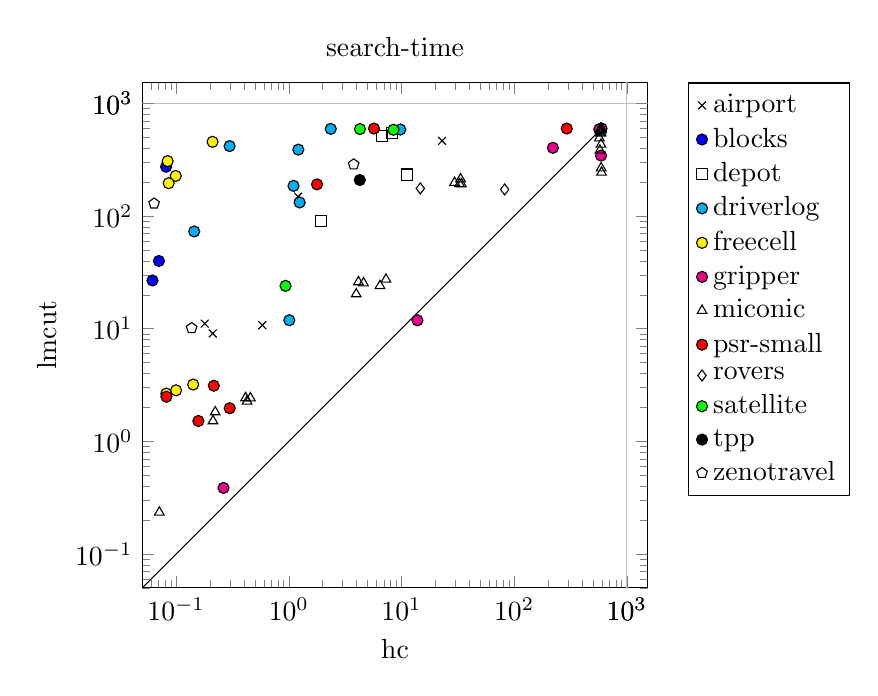
\begin{tikzpicture}
\begin{axis}[extra x tick style={grid=major}, extra x ticks=1000, extra y tick style={grid=major}, 
extra y ticks=1000, height=8.00cm, legend cell align=left, legend style={at={(1.4, 1)}}, title=search-time, width=8.00cm, xlabel=hc, xmin=0.05, xmode=log, ylabel=lmcut, ymin=0.05, ymode=log]
\addplot[color=green, mark=x, mark options={{draw=black}}, only marks] coordinates {
(0.010000, 0.145019) (0.179368, 11.087800) (0.010000, 0.148471) (22.919350, 465.248041) (0.010000, 0.138836) (1.207802, 148.594000) (0.580962, 10.739300) (0.010000, 0.010000) (0.010000, 0.144218) (0.211029, 9.069710)
};
\addlegendentry{airport}
\addplot[color=blue, mark=*, mark options={{draw=black}}, only marks] coordinates {
(0.010000, 0.241287) (0.081349, 273.943000) (0.032068, 25.498900) (0.024986, 17.856400) (0.010000, 0.013831) (0.010000, 0.011050) (0.010000, 0.014994) (0.070254, 39.917200) (0.011799, 1.396270) (0.031537, 2.845540) (0.038953, 56.848500) (0.010000, 0.010000) (0.061611, 26.801200) (0.010000, 0.084920) (0.010000, 0.143467) (0.010000, 0.053145)
};
\addlegendentry{blocks}
\addplot[color=magenta, mark=square, mark options={{draw=black}}, only marks] coordinates {
(8.306120, 546.413867) (0.010000, 0.454776) (0.010000, 0.010000) (11.217900, 233.682000) (6.757340, 513.742809) (1.943620, 90.322400)
};
\addlegendentry{depot}
\addplot[color=cyan, mark=*, mark options={{draw=black}}, only marks] coordinates {
(2.354820, 594.273762) (1.100020, 185.435000) (1.214180, 388.772000) (9.760760, 585.985461) (0.013146, 0.355551) (0.297981, 417.908000) (0.010000, 0.010000) (1.009640, 11.880900) (0.144535, 73.016200) (1.246790, 132.045000)
};
\addlegendentry{driverlog}
\addplot[color=yellow, mark=*, mark options={{draw=black}}, only marks] coordinates {
(0.099051, 227.105000) (0.083962, 307.362000) (0.210252, 455.826000) (0.042857, 2.234200) (0.010000, 0.197040) (0.099746, 2.836240) (0.037383, 2.066460) (0.085739, 195.725000) (0.013246, 14.349400) (0.081759, 2.653950) (0.025328, 255.793000) (0.141554, 3.192820)
};
\addlegendentry{freecell}
\addplot[color=magenta, mark=*, mark options={{draw=black}}, only marks] coordinates {
(591.089502, 344.121000) (0.262926, 0.385840) (596.647608, 599.519963) (569.492855, 589.232378) (13.844100, 11.876000) (220.812500, 403.291000) (0.010000, 0.014257)
};
\addlegendentry{gripper}
\addplot[color=cyan, mark=triangle, mark options={{draw=black}}, only marks] coordinates {
(7.282070, 27.391700) (590.112556, 432.887000) (0.212131, 1.517590) (0.425846, 2.264950) (32.738500, 192.940000) (0.222096, 1.820830) (584.148657, 587.696141) (0.026386, 0.169860) (577.370218, 579.753396) (0.048676, 0.217090) (596.722586, 243.971000) (586.187417, 543.923243) (0.455739, 2.420320) (585.890390, 587.271962) (0.039212, 0.219873) (592.930220, 585.958915) (4.148850, 26.007800) (570.608013, 491.997000) (0.010000, 0.030098) (0.010000, 0.028190) (0.042445, 0.204913) (585.482311, 597.641841) (4.599160, 25.405300) (6.442820, 24.030000) (590.819602, 595.781666) (0.010000, 0.027890) (592.167179, 266.793000) (33.443600, 213.065000) (596.108119, 593.064799) (0.010000, 0.029482) (0.070847, 0.234214) (34.077400, 192.393000) (0.412567, 2.426510) (3.963360, 20.321900) (586.905028, 579.938124) (29.592500, 197.966000) (588.228783, 555.366355) (0.010000, 0.010000) (0.010000, 0.028766) (577.634284, 383.340000)
};
\addlegendentry{miconic}
\addplot[color=red, mark=*, mark options={{draw=black}}, only marks] coordinates {
(0.215694, 3.116640) (0.022007, 0.131474) (0.157385, 1.515700) (0.010000, 0.063653) (0.010000, 0.015288) (5.700890, 597.876933) (0.010000, 0.439747) (0.034962, 0.159061) (0.010000, 0.014646) (0.020044, 0.123132) (0.014752, 0.084136) (0.010000, 0.013838) (0.010000, 0.010526) (293.244000, 598.462153) (0.010000, 0.057526) (0.011576, 0.033149) (0.020875, 0.073845) (0.010000, 0.035914) (0.016773, 0.010000) (0.081920, 2.488950) (1.779940, 191.082000) (0.010000, 0.014621) (0.010850, 0.058979) (0.010000, 0.032497) (0.298527, 1.967380) (0.030218, 0.126164) (0.010000, 0.010000) (0.013860, 0.053829) (0.010000, 0.043889)
};
\addlegendentry{psr-small}
\addplot[color=blue, mark=diamond, mark options={{draw=black}}, only marks] coordinates {
(14.684900, 175.966000) (0.010000, 0.012330) (82.362900, 172.156000) (0.010000, 0.010000)
};
\addlegendentry{rovers}
\addplot[color=green, mark=*, mark options={{draw=black}}, only marks] coordinates {
(0.010000, 0.037315) (0.935294, 24.005000) (8.485640, 583.323190) (0.016291, 0.290613) (4.278860, 591.951665) (0.010000, 0.010000)
};
\addlegendentry{satellite}
\addplot[color=black, mark=*, mark options={{draw=black}}, only marks] coordinates {
(0.010000, 0.021228) (0.010000, 0.010000) (0.033617, 0.729151) (4.261390, 208.745000)
};
\addlegendentry{tpp}
\addplot[color=red, mark=pentagon, mark options={{draw=black}}, only marks] coordinates {
(0.137054, 10.125700) (0.010000, 0.010000) (0.063638, 129.227000) (0.010000, 0.089784) (0.010000, 0.426249) (3.762470, 287.667000) (0.010000, 0.149214) (0.018711, 4.364840)
};
\addlegendentry{zenotravel}
\addplot[color=black] coordinates {(0.050000, 0.050000) (599, 599)};
\end{axis}
\end{tikzpicture}
\\
        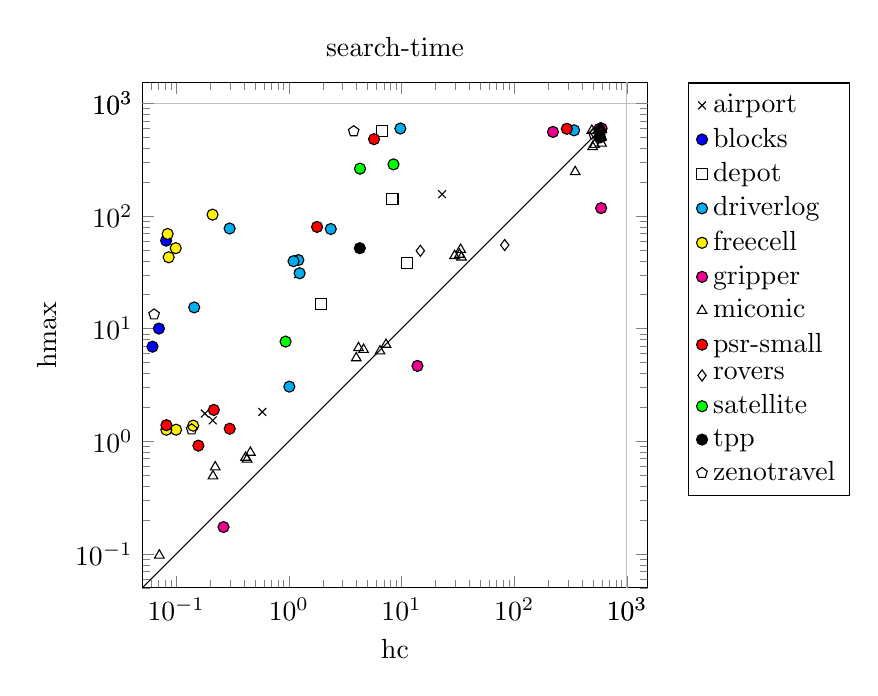
\begin{tikzpicture}
\begin{axis}[extra x tick style={grid=major}, extra x ticks=1000, extra y tick style={grid=major}, 
extra y ticks=1000, height=8.00cm, legend cell align=left, legend style={at={(1.4, 1)}}, title=search-time, width=8.00cm, xlabel=hc, xmin=0.05, xmode=log, ylabel=hmax, ymin=0.05, ymode=log]
\addplot[color=green, mark=x, mark options={{draw=black}}, only marks] coordinates {
(0.211029, 1.535550) (0.179368, 1.763850) (22.919350, 156.197000) (1.207802, 30.523000) (0.010000, 0.035344) (0.010000, 0.035362) (0.010000, 0.031154) (0.010000, 0.037047) (0.010000, 0.010000) (0.580962, 1.822400)
};
\addlegendentry{airport}
\addplot[color=blue, mark=*, mark options={{draw=black}}, only marks] coordinates {
(0.032068, 5.732710) (0.070254, 10.017100) (0.010000, 0.047037) (0.010000, 0.012368) (0.061611, 6.917790) (0.010000, 0.012243) (0.038953, 12.781400) (0.010000, 0.113656) (0.031537, 0.862602) (0.024986, 4.632420) (0.010000, 0.010000) (0.011799, 0.439723) (0.010000, 0.064324) (0.081349, 60.444000) (0.010000, 0.033449)
};
\addlegendentry{blocks}
\addplot[color=magenta, mark=square, mark options={{draw=black}}, only marks] coordinates {
(0.010000, 0.127047) (1.943620, 16.555100) (11.217900, 38.239000) (8.306120, 140.910000) (0.010000, 0.010000) (6.757340, 565.255782)
};
\addlegendentry{depot}
\addplot[color=cyan, mark=*, mark options={{draw=black}}, only marks] coordinates {
(0.297981, 77.459500) (9.760760, 597.749223) (0.013146, 0.115082) (2.354820, 76.663600) (1.009640, 3.057640) (0.144535, 15.437500) (1.246790, 31.041800) (1.214180, 40.615900) (0.010000, 0.010000) (1.100020, 39.711100) (340.116000, 575.892081)
};
\addlegendentry{driverlog}
\addplot[color=yellow, mark=*, mark options={{draw=black}}, only marks] coordinates {
(0.025328, 59.011600) (0.210252, 102.793000) (0.010000, 0.124281) (0.099746, 1.267980) (0.083962, 69.265900) (0.141554, 1.376880) (0.042857, 1.066010) (0.037383, 1.096480) (0.081759, 1.266610) (0.013246, 3.938400) (0.099051, 51.804200) (0.085739, 43.038000)
};
\addlegendentry{freecell}
\addplot[color=magenta, mark=*, mark options={{draw=black}}, only marks] coordinates {
(13.844100, 4.669780) (596.647608, 598.667659) (591.089502, 117.455000) (0.262926, 0.173503) (569.492855, 593.108070) (0.010000, 0.010000) (220.812500, 557.649400)
};
\addlegendentry{gripper}
\addplot[color=cyan, mark=triangle, mark options={{draw=black}}, only marks] coordinates {
(0.425846, 0.692233) (4.599160, 6.511650) (588.228783, 591.122512) (0.212131, 0.491115) (3.963360, 5.488040) (6.442820, 6.315310) (517.980280, 429.754000) (0.048676, 0.089155) (0.455739, 0.795860) (577.634284, 561.149300) (347.818020, 246.674000) (0.222096, 0.591140) (0.070847, 0.097298) (577.370218, 598.055292) (34.077400, 43.061700) (29.592500, 44.360300) (4.148850, 6.747270) (592.167179, 595.122680) (596.722586, 585.635170) (592.930220, 499.164000) (586.905028, 594.884152) (590.112556, 578.235044) (596.108119, 441.372000) (549.845320, 569.778350) (0.010000, 0.014717) (33.443600, 50.381600) (0.412567, 0.717870) (585.482311, 493.436000) (586.187417, 592.331096) (0.039212, 0.088437) (594.301000, 509.525200) (0.010000, 0.015111) (488.742600, 574.346900) (570.608013, 589.738525) (584.148657, 595.027433) (0.026386, 0.071008) (585.890390, 494.009000) (496.366840, 410.867000) (0.010000, 0.014640) (7.282070, 7.229640) (0.010000, 0.015968) (590.819602, 595.820423) (0.042445, 0.083550) (0.010000, 0.010000) (32.738500, 45.512700) (0.010000, 0.014809)
};
\addlegendentry{miconic}
\addplot[color=red, mark=*, mark options={{draw=black}}, only marks] coordinates {
(0.022007, 0.186275) (0.010000, 0.013324) (0.010850, 0.048356) (0.010000, 0.046423) (0.010000, 0.062220) (0.013860, 0.058309) (0.010000, 0.021642) (0.020044, 0.096882) (0.010000, 0.045396) (0.010000, 0.012186) (5.700890, 480.711000) (1.779940, 80.007200) (0.215694, 1.899360) (0.030218, 0.140215) (0.020875, 0.055608) (0.010000, 0.017516) (0.034962, 0.155076) (0.011576, 0.011249) (0.010000, 0.012182) (0.010000, 0.045889) (0.010000, 0.010726) (0.010000, 0.013610) (0.016773, 0.010000) (0.010000, 0.020060) (0.010000, 0.018839) (0.014752, 0.110608) (293.244000, 594.306057) (0.081920, 1.389790) (0.157385, 0.915276) (0.298527, 1.293440) (0.010000, 0.010000) (0.010000, 0.038902)
};
\addlegendentry{psr-small}
\addplot[color=blue, mark=diamond, mark options={{draw=black}}, only marks] coordinates {
(82.362900, 55.198900) (511.206762, 551.957520) (14.684900, 49.125200) (0.010000, 0.010000)
};
\addlegendentry{rovers}
\addplot[color=green, mark=*, mark options={{draw=black}}, only marks] coordinates {
(0.016291, 0.140580) (0.010000, 0.021659) (0.935294, 7.679300) (4.278860, 263.238000) (0.010000, 0.010000) (8.485640, 287.232000)
};
\addlegendentry{satellite}
\addplot[color=black, mark=*, mark options={{draw=black}}, only marks] coordinates {
(576.817000, 498.468930) (0.033617, 0.280404) (4.261390, 51.802300) (0.010000, 0.010000) (0.010000, 0.013405)
};
\addlegendentry{tpp}
\addplot[color=red, mark=pentagon, mark options={{draw=black}}, only marks] coordinates {
(0.010000, 0.066958) (3.762470, 565.487054) (511.621367, 529.978709) (0.063638, 13.368700) (0.137054, 1.276830) (0.010000, 0.036161) (0.010000, 0.010000) (0.010000, 0.046869) (0.018711, 0.643291)
};
\addlegendentry{zenotravel}
\addplot[color=black] coordinates {(0.050000, 0.050000) (598, 598)};
\end{axis}
\end{tikzpicture}
\\
        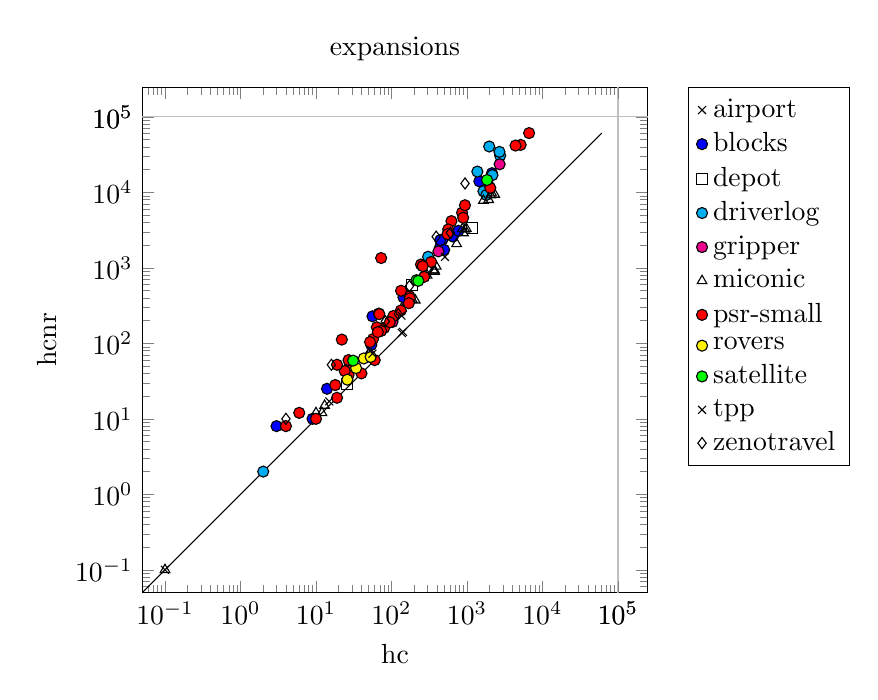
\begin{tikzpicture}
\begin{axis}[extra x tick style={grid=major}, extra x ticks=100000, extra y tick style={grid=major}, 
extra y ticks=100000, height=8.00cm, legend cell align=left, legend style={at={(1.4, 1)}}, title=expansions, width=8.00cm, xlabel=hc, xmin=0.05, xmode=log, ylabel=hcnr, ymin=0.05, ymode=log]
\addplot[color=red, mark=x, mark options={{draw=black}}, only marks] coordinates {
(0.100000, 0.100000) (137, 137) (142, 142)
};
\addlegendentry{airport}
\addplot[color=blue, mark=*, mark options={{draw=black}}, only marks] coordinates {
(100, 202) (1875, 13298) (2144, 17941) (439, 1855) (651, 2599) (3, 8) (14, 25) (499, 1732) (144, 407) (56, 228) (9, 10) (106, 219) (1458, 14012) (474, 2375) (70, 149) (54, 95) (770, 3093) (442, 2329)
};
\addlegendentry{blocks}
\addplot[color=cyan, mark=square, mark options={{draw=black}}, only marks] coordinates {
(1165, 3337) (26, 29) (186, 594)
};
\addlegendentry{depot}
\addplot[color=cyan, mark=*, mark options={{draw=black}}, only marks] coordinates {
(2176, 16918) (1652, 10340) (1805, 9221) (306, 1402) (1971, 40492) (2, 2) (2754, 30702) (1373, 18842) (2695, 34370)
};
\addlegendentry{driverlog}
\addplot[color=magenta, mark=*, mark options={{draw=black}}, only marks] coordinates {
(103, 192) (2708, 23542) (419, 1653)
};
\addlegendentry{gripper}
\addplot[color=blue, mark=triangle, mark options={{draw=black}}, only marks] coordinates {
(981, 3311) (1651, 7795) (188, 381) (2121, 9781) (12, 12) (371, 930) (730, 2078) (52, 77) (372, 890) (1940, 7993) (48, 63) (359, 929) (10, 12) (937, 3229) (51, 66) (164, 345) (0.100000, 0.100000) (47, 66) (46, 62) (13, 15) (2333, 9377) (296, 797) (391, 1046) (136, 290) (207, 372) (901, 2892) (2060, 9235) (867, 3283) (164, 351)
};
\addlegendentry{miconic}
\addplot[color=red, mark=*, mark options={{draw=black}}, only marks] coordinates {
(271, 760) (19, 19) (4, 8) (28, 55) (106, 230) (22, 112) (173, 421) (246, 1106) (27, 38) (5143, 42522) (68, 248) (27, 60) (861, 5382) (891, 4609) (60, 60) (80, 160) (64, 163) (6652, 60966) (24, 43) (57, 114) (73, 1348) (175, 395) (69, 244) (623, 4157) (18, 28) (52, 104) (73, 146) (6, 12) (2036, 11460) (95, 190) (134, 497) (564, 3227) (133, 272) (10, 10) (552, 2794) (335, 1194) (66, 141) (40, 40) (259, 1053) (941, 6750) (4401, 41680) (19, 52) (170, 340)
};
\addlegendentry{psr-small}
\addplot[color=yellow, mark=*, mark options={{draw=black}}, only marks] coordinates {
(34, 47) (43, 63) (53, 66) (26, 33)
};
\addlegendentry{rovers}
\addplot[color=green, mark=*, mark options={{draw=black}}, only marks] coordinates {
(214, 686) (227, 673) (1844, 14576) (31, 59)
};
\addlegendentry{satellite}
\addplot[color=green, mark=x, mark options={{draw=black}}, only marks] coordinates {
(56, 73) (136, 233) (511, 1394) (15, 17)
};
\addlegendentry{tpp}
\addplot[color=black, mark=diamond, mark options={{draw=black}}, only marks] coordinates {
(942, 13116) (123, 244) (4, 10) (173, 573) (16, 52) (602, 2919) (391, 2589) (83, 195)
};
\addlegendentry{zenotravel}
\addplot[color=black] coordinates {(0.050000, 0.050000) (60966, 60966)};
\end{axis}
\end{tikzpicture}
\\
        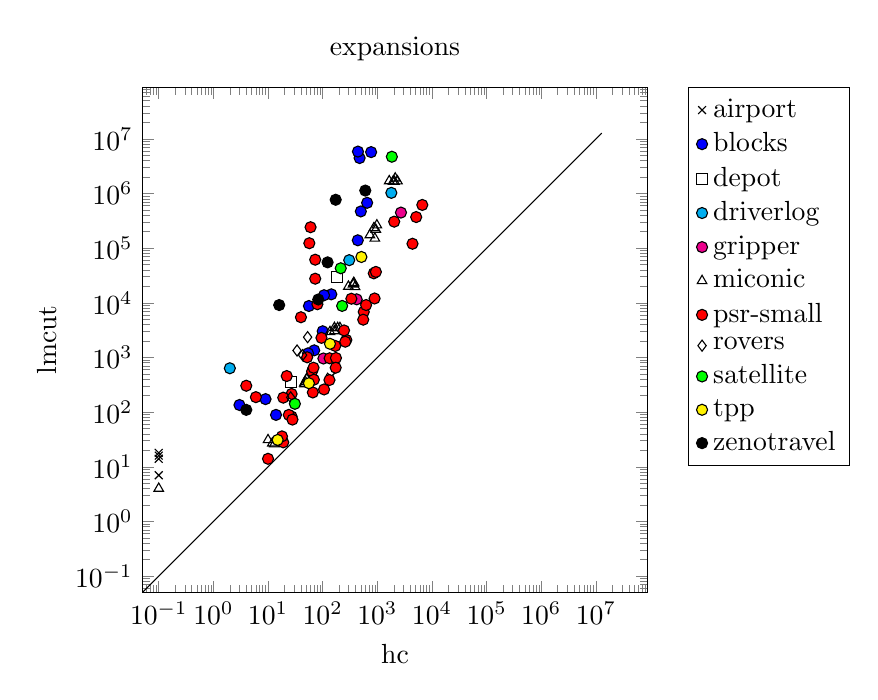
\begin{tikzpicture}
\begin{axis}[extra x tick style={grid=major}, extra x ticks=100000000, extra y tick style={grid=major}, extra y ticks=100000000, height=8.00cm, 
legend cell align=left, legend style={at={(1.4, 1)}}, title=expansions, width=8.00cm, xlabel=hc, xmin=0.05, xmode=log, ylabel=lmcut, ymin=0.05, ymode=log]
\addplot[color=red, mark=x, mark options={{draw=black}}, only marks] coordinates {
(142, 444) (0.100000, 14) (0.100000, 18) (0.100000, 7) (0.100000, 16) (137, 421)
};
\addlegendentry{airport}
\addplot[color=blue, mark=*, mark options={{draw=black}}, only marks] coordinates {
(9, 173) (474, 4460545) (100, 3018) (439, 139356) (14, 89) (144, 14312) (442, 5854588) (106, 13778) (56, 8750) (651, 676067) (770, 5723779) (3, 135) (70, 1350) (54, 1191) (499, 470462)
};
\addlegendentry{blocks}
\addplot[color=cyan, mark=square, mark options={{draw=black}}, only marks] coordinates {
(186, 30045) (26, 362)
};
\addlegendentry{depot}
\addplot[color=cyan, mark=*, mark options={{draw=black}}, only marks] coordinates {
(306, 60344) (1805, 1028572) (2, 635)
};
\addlegendentry{driverlog}
\addplot[color=magenta, mark=*, mark options={{draw=black}}, only marks] coordinates {
(103, 958) (419, 11586) (2708, 448198)
};
\addlegendentry{gripper}
\addplot[color=blue, mark=triangle, mark options={{draw=black}}, only marks] coordinates {
(2121, 1903853) (372, 22499) (48, 361) (13, 26) (52, 424) (391, 19586) (1940, 1650838) (12, 27) (730, 174147) (1651, 1697048) (51, 400) (2333, 1690274) (47, 327) (901, 151003) (359, 21853) (10, 31) (188, 3492) (46, 336) (371, 23396) (981, 263639) (207, 3488) (296, 19955) (0.100000, 4) (164, 3060) (867, 234915) (136, 2947) (937, 219412) (164, 3501) (2060, 1656771)
};
\addlegendentry{miconic}
\addplot[color=red, mark=*, mark options={{draw=black}}, only marks] coordinates {
(271, 2092) (27, 215) (861, 34633) (64, 557) (27, 83) (40, 5446) (80, 9432) (564, 6833) (73, 27640) (73, 61548) (6652, 618078) (259, 1944) (106, 260) (4401, 120468) (4, 304) (24, 89) (10, 14) (19, 28) (52, 1008) (623, 9112) (28, 73) (57, 123268) (95, 2286) (891, 12005) (552, 4917) (22, 457) (134, 967) (69, 392) (133, 387) (68, 649) (60, 241899) (335, 11892) (6, 188) (5143, 370920) (18, 36) (19, 184) (170, 1626) (175, 979) (66, 229) (941, 36799) (173, 650) (246, 3125) (2036, 305520)
};
\addlegendentry{psr-small}
\addplot[color=green, mark=diamond, mark options={{draw=black}}, only marks] coordinates {
(34, 1343) (43, 1106) (53, 2354) (26, 186)
};
\addlegendentry{rovers}
\addplot[color=green, mark=*, mark options={{draw=black}}, only marks] coordinates {
(214, 42892) (31, 142) (227, 8777) (1844, 4711577)
};
\addlegendentry{satellite}
\addplot[color=yellow, mark=*, mark options={{draw=black}}, only marks] coordinates {
(511, 69014) (136, 1779) (15, 31) (56, 338)
};
\addlegendentry{tpp}
\addplot[color=black, mark=*, mark options={{draw=black}}, only marks] coordinates {
(602, 1133103) (16, 9104) (4, 110) (123, 55014) (83, 11510) (173, 769022)
};
\addlegendentry{zenotravel}
\addplot[color=black] coordinates {(0.050000, 0.050000) (12763448, 12763448)};
\end{axis}
\end{tikzpicture}
\\
        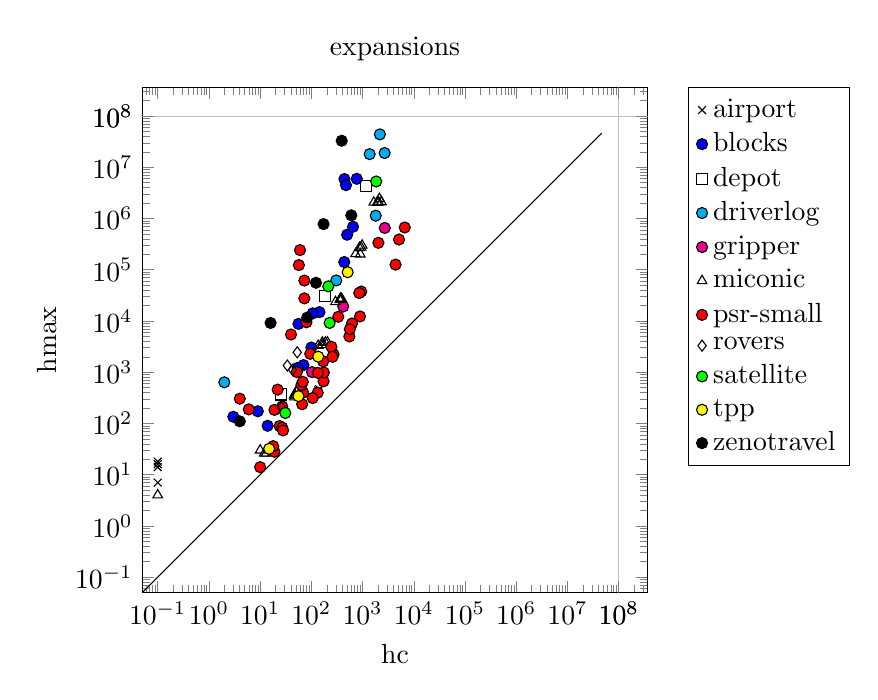
\begin{tikzpicture}
\begin{axis}[extra x tick style={grid=major}, extra x ticks=100000000, extra y tick style={grid=major}, extra y ticks=100000000, height=8.00cm,
 legend cell align=left, legend style={at={(1.4, 1)}}, title=expansions, width=8.00cm, xlabel=hc, xmin=0.05, xmode=log, ylabel=hmax, ymin=0.05, ymode=log]
\addplot[color=red, mark=x, mark options={{draw=black}}, only marks] coordinates {
(142, 464) (0.100000, 14) (0.100000, 18) (0.100000, 7) (0.100000, 16) (137, 441)
};
\addlegendentry{airport}
\addplot[color=blue, mark=*, mark options={{draw=black}}, only marks] coordinates {
(144, 14897) (9, 173) (442, 5894179) (70, 1376) (499, 483086) (56, 8783) (439, 141443) (100, 3031) (14, 90) (3, 135) (474, 4487213) (54, 1215) (651, 691186) (106, 14089) (770, 5968890)
};
\addlegendentry{blocks}
\addplot[color=cyan, mark=square, mark options={{draw=black}}, only marks] coordinates {
(186, 30239) (1165, 4348281) (26, 368)
};
\addlegendentry{depot}
\addplot[color=cyan, mark=*, mark options={{draw=black}}, only marks] coordinates {
(306, 61958) (1373, 18078718) (2695, 19007847) (1805, 1136659) (2, 635) (2176, 43967863)
};
\addlegendentry{driverlog}
\addplot[color=magenta, mark=*, mark options={{draw=black}}, only marks] coordinates {
(419, 19191) (103, 1006) (2708, 655342)
};
\addlegendentry{gripper}
\addplot[color=blue, mark=triangle, mark options={{draw=black}}, only marks] coordinates {
(51, 424) (372, 27235) (207, 3838) (13, 26) (1940, 2054791) (2333, 2104717) (48, 359) (10, 30) (188, 3838) (164, 3428) (46, 353) (47, 327) (730, 203857) (0.100000, 4) (981, 299347) (901, 201439) (937, 273423) (867, 269792) (136, 3311) (391, 27181) (371, 27525) (1651, 2066634) (296, 23696) (2121, 2441914) (2060, 2086171) (12, 26) (164, 3838) (52, 422) (359, 25847)
};
\addlegendentry{miconic}
\addplot[color=red, mark=*, mark options={{draw=black}}, only marks] coordinates {
(27, 215) (552, 4995) (133, 397) (335, 12092) (66, 237) (623, 8950) (40, 5446) (80, 9432) (73, 27640) (73, 61548) (271, 2230) (69, 400) (106, 313) (4, 304) (24, 89) (5143, 389358) (10, 14) (52, 1008) (19, 28) (57, 123268) (173, 665) (95, 2286) (891, 12261) (4401, 126004) (27, 83) (64, 561) (22, 457) (564, 6921) (6652, 668998) (175, 987) (68, 649) (60, 241899) (246, 3131) (6, 188) (134, 970) (28, 73) (18, 36) (2036, 335904) (19, 184) (170, 1626) (259, 2000) (941, 37611) (861, 35149)
};
\addlegendentry{psr-small}
\addplot[color=green, mark=diamond, mark options={{draw=black}}, only marks] coordinates {
(26, 207) (34, 1350) (53, 2442) (43, 1113)
};
\addlegendentry{rovers}
\addplot[color=green, mark=*, mark options={{draw=black}}, only marks] coordinates {
(227, 9176) (214, 47435) (1844, 5287951) (31, 160)
};
\addlegendentry{satellite}
\addplot[color=yellow, mark=*, mark options={{draw=black}}, only marks] coordinates {
(511, 89604) (56, 341) (15, 32) (136, 2013)
};
\addlegendentry{tpp}
\addplot[color=black, mark=*, mark options={{draw=black}}, only marks] coordinates {
(4, 110) (16, 9148) (123, 55748) (602, 1155505) (83, 11658) (391, 33028328) (173, 778708)
};
\addlegendentry{zenotravel}
\addplot[color=black] coordinates {(0.050000, 0.050000) (46590097, 46590097)};
\end{axis}
\end{tikzpicture}

    \end{center}


    \subsubsection*{Cost Bound 0.75}

    \begin{center}

        \begin{tabular}{l|r|r|r|r}
            Finished PPD1 & hc & hcnr & hmax & lmcut \\\hline
            airport (19) & 8 & 8 & \textbf{16} & 15\\\hline
            blocks (18) & \textbf{18} & \textbf{18} & 15 & 15 \\\hline
            depot (6) & 3 & 3 & \textbf{4} & 2 \\\hline
            driverlog (11) & \textbf{9} & \textbf{9} & 6 & 3 \\\hline
            freecell (55) & 0 & 0 & \textbf{13} & 7 \\\hline
            gripper (8) & 3 & 3 & \textbf{4} & \textbf{4} \\\hline
            miconic (69) & 35 & \textbf{39} & \textbf{39} & \textbf{39} \\\hline
            PSR (49) & \textbf{47} & 45 & 46 & 46 \\\hline
            rovers (7) & 4 & 5 & \textbf{6} & 4 \\\hline
            satellite (6) & 4 & \textbf{5} & 4 & 4 \\\hline
            tpp (10) & 4 & \textbf{5} & \textbf{5} & 4 \\\hline
            zenotravel (11) & \textbf{8} & \textbf{8} & 7 & 6 \\\hline\hline
            sum (269) & 143 & 148 & \textbf{165} & 149 \\
        \end{tabular}

        \scriptsize
        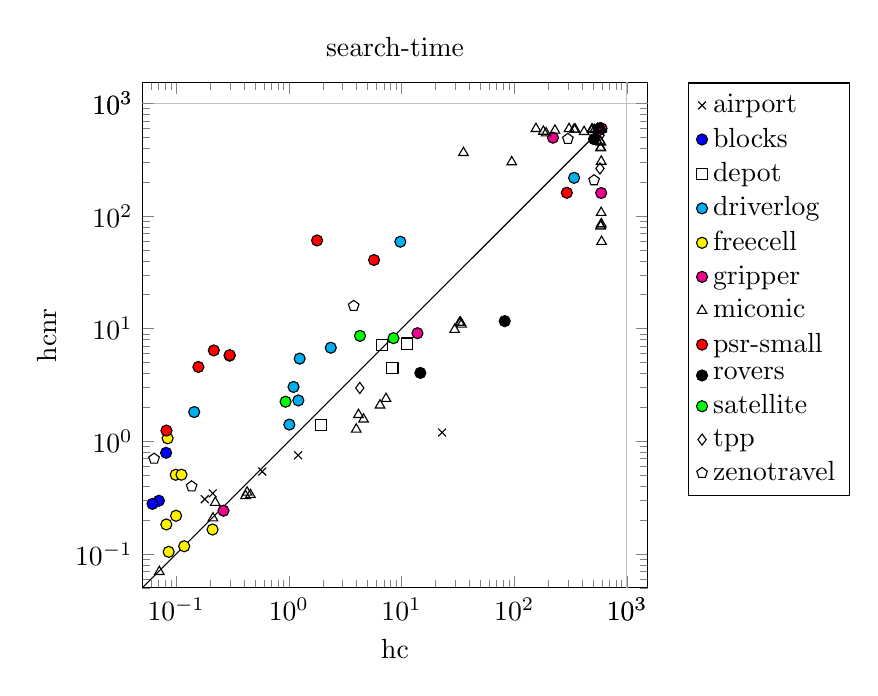
\begin{tikzpicture}
\begin{axis}[extra x tick style={grid=major}, extra x ticks=1000, extra y tick style={grid=major}, 
extra y ticks=1000, height=8cm, legend cell align=left, legend style={at={(1.4, 1)}}, title=search-time, width=8cm, xlabel=hc, xmin=0.05, xmode=log, ylabel=hcnr, ymin=0.05, ymode=log]
\addplot[color=green, mark=x, mark options={{draw=black}}, only marks] coordinates {
(0.580962, 0.539156) (22.919350, 1.197450) (1.207802, 0.751533) (0.010000, 0.010000) (0.211029, 0.344864) (0.179368, 0.306256)
};
\addlegendentry{airport}
\addplot[color=blue, mark=*, mark options={{draw=black}}, only marks] coordinates {
(0.070254, 0.296864) (0.031537, 0.132323) (0.061611, 0.278351) (0.010000, 0.015546) (0.081349, 0.790786) (0.032068, 0.459737) (0.010000, 0.022621) (0.038953, 0.506324) (0.024986, 0.185765) (0.010000, 0.019080) (0.010000, 0.010000) (0.010000, 0.045402) (0.011799, 0.083719)
};
\addlegendentry{blocks}
\addplot[color=magenta, mark=square, mark options={{draw=black}}, only marks] coordinates {
(11.217900, 7.372310) (0.010000, 0.032782) (6.757340, 7.158310) (0.010000, 0.010000) (8.306120, 4.493250) (1.943620, 1.390270)
};
\addlegendentry{depot}
\addplot[color=cyan, mark=*, mark options={{draw=black}}, only marks] coordinates {
(0.297981, 5.756450) (0.144535, 1.819230) (1.100020, 3.040280) (1.214180, 2.305950) (340.116000, 218.241000) (9.760760, 59.133700) (1.246790, 5.421790) (1.009640, 1.408210) (0.013146, 0.044778) (0.010000, 0.010000) (2.354820, 6.773570)
};
\addlegendentry{driverlog}
\addplot[color=yellow, mark=*, mark options={{draw=black}}, only marks] coordinates {
(0.099746, 0.218327) (0.210252, 0.164829) (0.042857, 0.142258) (0.013246, 0.016653) (0.117766, 0.117104) (0.099051, 0.504578) (0.083962, 1.063150) (0.010000, 0.023282) (0.037383, 0.106107) (0.141554, 0.013294) (0.081759, 0.182805) (0.111385, 0.505483) (0.025328, 0.024882) (0.085739, 0.104453)
};
\addlegendentry{freecell}
\addplot[color=magenta, mark=*, mark options={{draw=black}}, only marks] coordinates {
(0.262926, 0.241988) (220.812500, 495.988300) (596.647608, 597.565062) (569.492855, 580.212440) (0.010000, 0.010000) (13.844100, 9.110310) (591.089502, 160.080000)
};
\addlegendentry{gripper}
\addplot[color=cyan, mark=triangle, mark options={{draw=black}}, only marks] coordinates {
(339.622700, 588.378030) (0.010000, 0.011511) (549.845320, 596.864944) (590.112556, 597.189862) (7.282070, 2.391340) (0.010000, 0.012300) (0.412567, 0.327916) (584.148657, 401.133000) (6.442820, 2.091980) (0.039212, 0.046379) (3.963360, 1.277520) (590.819602, 107.059000) (586.187417, 597.268517) (306.656100, 594.349870) (95.053000, 301.677300) (34.077400, 10.919400) (181.635500, 562.785100) (0.010000, 0.012302) (35.450700, 364.431800) (594.301000, 589.966394) (592.930220, 85.041900) (585.482311, 81.044100) (0.026386, 0.042528) (570.608013, 597.167369) (347.818020, 587.793298) (155.906400, 595.750950) (32.738500, 11.323200) (596.722586, 598.978263) (0.070847, 0.069548) (191.937600, 544.281070) (577.370218, 460.882000) (496.366840, 586.208798) (0.042445, 0.049317) (592.167179, 305.104556) (0.455739, 0.335505) (29.592500, 9.804140) (0.048676, 0.049344) (4.148850, 1.722520) (585.890390, 82.624400) (0.212131, 0.208158) (586.905028, 407.188000) (577.634284, 595.238650) (588.228783, 451.849000) (517.980280, 582.901515) (0.222096, 0.285741) (488.742600, 588.815017) (596.108119, 59.254000) (229.859700, 575.452420) (4.599160, 1.569080) (0.010000, 0.010000) (33.443600, 11.359900) (0.425846, 0.352192) (417.259400, 559.410200) (0.010000, 0.012175)
};
\addlegendentry{miconic}
\addplot[color=red, mark=*, mark options={{draw=black}}, only marks] coordinates {
(0.010000, 0.011470) (0.010000, 0.032399) (293.244000, 160.887713) (0.010000, 0.012510) (0.020875, 0.200436) (0.215694, 6.411470) (0.010000, 0.019380) (0.081920, 1.245030) (0.013860, 0.108072) (0.034962, 0.448613) (0.020044, 0.175404) (0.157385, 4.569860) (0.010000, 0.044764) (0.011576, 0.024512) (0.298527, 5.820420) (0.010000, 0.010334) (0.010000, 0.058066) (1.779940, 60.661200) (0.010000, 0.020175) (0.030218, 0.282279) (0.014752, 0.078198) (0.010000, 0.010393) (0.010000, 0.031036) (0.010850, 0.076801) (0.010000, 0.015075) (0.016773, 0.031202) (0.022007, 0.111476) (0.010000, 0.010273) (0.010000, 0.010000) (5.700890, 40.694000)
};
\addlegendentry{psr-small}
\addplot[color=black, mark=*, mark options={{draw=black}}, only marks] coordinates {
(14.684900, 4.047890) (82.362900, 11.664700) (511.206762, 481.269259) (0.010000, 0.010000)
};
\addlegendentry{rovers}
\addplot[color=green, mark=*, mark options={{draw=black}}, only marks] coordinates {
(8.485640, 8.230840) (0.016291, 0.046241) (0.935294, 2.246410) (0.010000, 0.010000) (0.010000, 0.027242) (4.278860, 8.627940)
};
\addlegendentry{satellite}
\addplot[color=blue, mark=diamond, mark options={{draw=black}}, only marks] coordinates {
(578.425608, 519.404647) (4.261390, 2.976200) (0.033617, 0.096048) (576.817000, 264.094000) (0.010000, 0.010000)
};
\addlegendentry{tpp}
\addplot[color=red, mark=pentagon, mark options={{draw=black}}, only marks] coordinates {
(511.621367, 207.755000) (0.018711, 0.085917) (553.269035, 596.441548) (0.010000, 0.020608) (0.063638, 0.701225) (3.762470, 15.939800) (0.010000, 0.010000) (0.010000, 0.016045) (0.010000, 0.011999) (0.137054, 0.398511) (299.509103, 483.854610)
};
\addlegendentry{zenotravel}
\addplot[color=black] coordinates {(0.050000, 0.050000) (598, 598)};
\end{axis}
\end{tikzpicture}
\\
        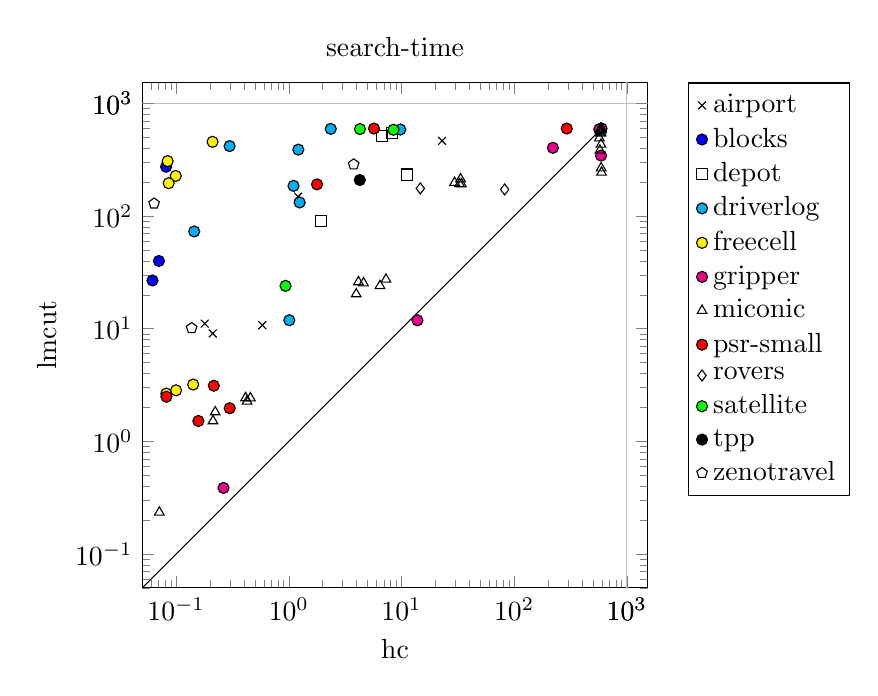
\begin{tikzpicture}
\begin{axis}[extra x tick style={grid=major}, extra x ticks=1000, extra y tick style={grid=major}, 
extra y ticks=1000, height=8.00cm, legend cell align=left, legend style={at={(1.4, 1)}}, title=search-time, width=8.00cm, xlabel=hc, xmin=0.05, xmode=log, ylabel=lmcut, ymin=0.05, ymode=log]
\addplot[color=green, mark=x, mark options={{draw=black}}, only marks] coordinates {
(0.010000, 0.145019) (0.179368, 11.087800) (0.010000, 0.148471) (22.919350, 465.248041) (0.010000, 0.138836) (1.207802, 148.594000) (0.580962, 10.739300) (0.010000, 0.010000) (0.010000, 0.144218) (0.211029, 9.069710)
};
\addlegendentry{airport}
\addplot[color=blue, mark=*, mark options={{draw=black}}, only marks] coordinates {
(0.010000, 0.241287) (0.081349, 273.943000) (0.032068, 25.498900) (0.024986, 17.856400) (0.010000, 0.013831) (0.010000, 0.011050) (0.010000, 0.014994) (0.070254, 39.917200) (0.011799, 1.396270) (0.031537, 2.845540) (0.038953, 56.848500) (0.010000, 0.010000) (0.061611, 26.801200) (0.010000, 0.084920) (0.010000, 0.143467) (0.010000, 0.053145)
};
\addlegendentry{blocks}
\addplot[color=magenta, mark=square, mark options={{draw=black}}, only marks] coordinates {
(8.306120, 546.413867) (0.010000, 0.454776) (0.010000, 0.010000) (11.217900, 233.682000) (6.757340, 513.742809) (1.943620, 90.322400)
};
\addlegendentry{depot}
\addplot[color=cyan, mark=*, mark options={{draw=black}}, only marks] coordinates {
(2.354820, 594.273762) (1.100020, 185.435000) (1.214180, 388.772000) (9.760760, 585.985461) (0.013146, 0.355551) (0.297981, 417.908000) (0.010000, 0.010000) (1.009640, 11.880900) (0.144535, 73.016200) (1.246790, 132.045000)
};
\addlegendentry{driverlog}
\addplot[color=yellow, mark=*, mark options={{draw=black}}, only marks] coordinates {
(0.099051, 227.105000) (0.083962, 307.362000) (0.210252, 455.826000) (0.042857, 2.234200) (0.010000, 0.197040) (0.099746, 2.836240) (0.037383, 2.066460) (0.085739, 195.725000) (0.013246, 14.349400) (0.081759, 2.653950) (0.025328, 255.793000) (0.141554, 3.192820)
};
\addlegendentry{freecell}
\addplot[color=magenta, mark=*, mark options={{draw=black}}, only marks] coordinates {
(591.089502, 344.121000) (0.262926, 0.385840) (596.647608, 599.519963) (569.492855, 589.232378) (13.844100, 11.876000) (220.812500, 403.291000) (0.010000, 0.014257)
};
\addlegendentry{gripper}
\addplot[color=cyan, mark=triangle, mark options={{draw=black}}, only marks] coordinates {
(7.282070, 27.391700) (590.112556, 432.887000) (0.212131, 1.517590) (0.425846, 2.264950) (32.738500, 192.940000) (0.222096, 1.820830) (584.148657, 587.696141) (0.026386, 0.169860) (577.370218, 579.753396) (0.048676, 0.217090) (596.722586, 243.971000) (586.187417, 543.923243) (0.455739, 2.420320) (585.890390, 587.271962) (0.039212, 0.219873) (592.930220, 585.958915) (4.148850, 26.007800) (570.608013, 491.997000) (0.010000, 0.030098) (0.010000, 0.028190) (0.042445, 0.204913) (585.482311, 597.641841) (4.599160, 25.405300) (6.442820, 24.030000) (590.819602, 595.781666) (0.010000, 0.027890) (592.167179, 266.793000) (33.443600, 213.065000) (596.108119, 593.064799) (0.010000, 0.029482) (0.070847, 0.234214) (34.077400, 192.393000) (0.412567, 2.426510) (3.963360, 20.321900) (586.905028, 579.938124) (29.592500, 197.966000) (588.228783, 555.366355) (0.010000, 0.010000) (0.010000, 0.028766) (577.634284, 383.340000)
};
\addlegendentry{miconic}
\addplot[color=red, mark=*, mark options={{draw=black}}, only marks] coordinates {
(0.215694, 3.116640) (0.022007, 0.131474) (0.157385, 1.515700) (0.010000, 0.063653) (0.010000, 0.015288) (5.700890, 597.876933) (0.010000, 0.439747) (0.034962, 0.159061) (0.010000, 0.014646) (0.020044, 0.123132) (0.014752, 0.084136) (0.010000, 0.013838) (0.010000, 0.010526) (293.244000, 598.462153) (0.010000, 0.057526) (0.011576, 0.033149) (0.020875, 0.073845) (0.010000, 0.035914) (0.016773, 0.010000) (0.081920, 2.488950) (1.779940, 191.082000) (0.010000, 0.014621) (0.010850, 0.058979) (0.010000, 0.032497) (0.298527, 1.967380) (0.030218, 0.126164) (0.010000, 0.010000) (0.013860, 0.053829) (0.010000, 0.043889)
};
\addlegendentry{psr-small}
\addplot[color=blue, mark=diamond, mark options={{draw=black}}, only marks] coordinates {
(14.684900, 175.966000) (0.010000, 0.012330) (82.362900, 172.156000) (0.010000, 0.010000)
};
\addlegendentry{rovers}
\addplot[color=green, mark=*, mark options={{draw=black}}, only marks] coordinates {
(0.010000, 0.037315) (0.935294, 24.005000) (8.485640, 583.323190) (0.016291, 0.290613) (4.278860, 591.951665) (0.010000, 0.010000)
};
\addlegendentry{satellite}
\addplot[color=black, mark=*, mark options={{draw=black}}, only marks] coordinates {
(0.010000, 0.021228) (0.010000, 0.010000) (0.033617, 0.729151) (4.261390, 208.745000)
};
\addlegendentry{tpp}
\addplot[color=red, mark=pentagon, mark options={{draw=black}}, only marks] coordinates {
(0.137054, 10.125700) (0.010000, 0.010000) (0.063638, 129.227000) (0.010000, 0.089784) (0.010000, 0.426249) (3.762470, 287.667000) (0.010000, 0.149214) (0.018711, 4.364840)
};
\addlegendentry{zenotravel}
\addplot[color=black] coordinates {(0.050000, 0.050000) (599, 599)};
\end{axis}
\end{tikzpicture}
\\
        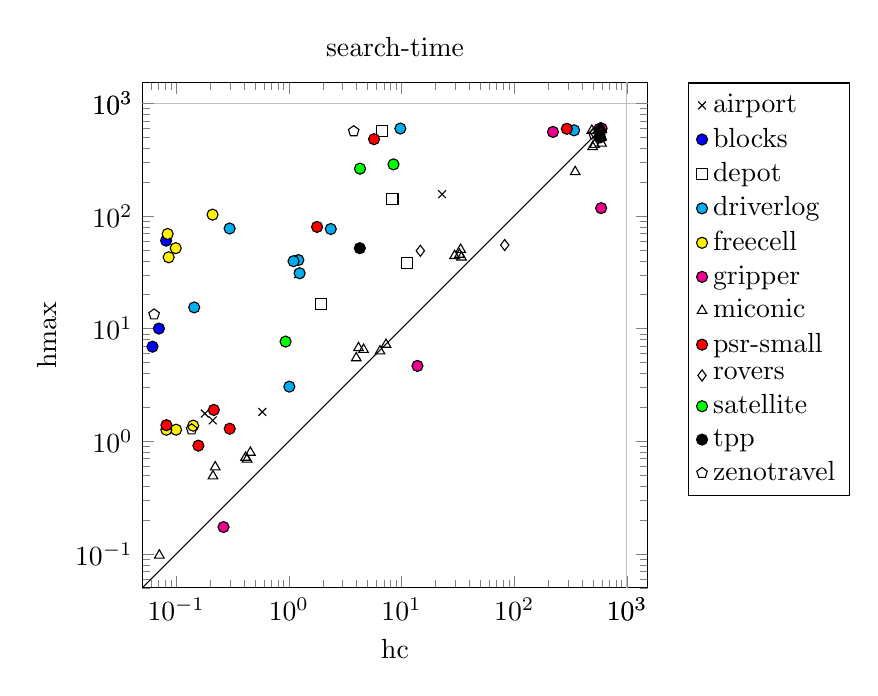
\begin{tikzpicture}
\begin{axis}[extra x tick style={grid=major}, extra x ticks=1000, extra y tick style={grid=major}, 
extra y ticks=1000, height=8.00cm, legend cell align=left, legend style={at={(1.4, 1)}}, title=search-time, width=8.00cm, xlabel=hc, xmin=0.05, xmode=log, ylabel=hmax, ymin=0.05, ymode=log]
\addplot[color=green, mark=x, mark options={{draw=black}}, only marks] coordinates {
(0.211029, 1.535550) (0.179368, 1.763850) (22.919350, 156.197000) (1.207802, 30.523000) (0.010000, 0.035344) (0.010000, 0.035362) (0.010000, 0.031154) (0.010000, 0.037047) (0.010000, 0.010000) (0.580962, 1.822400)
};
\addlegendentry{airport}
\addplot[color=blue, mark=*, mark options={{draw=black}}, only marks] coordinates {
(0.032068, 5.732710) (0.070254, 10.017100) (0.010000, 0.047037) (0.010000, 0.012368) (0.061611, 6.917790) (0.010000, 0.012243) (0.038953, 12.781400) (0.010000, 0.113656) (0.031537, 0.862602) (0.024986, 4.632420) (0.010000, 0.010000) (0.011799, 0.439723) (0.010000, 0.064324) (0.081349, 60.444000) (0.010000, 0.033449)
};
\addlegendentry{blocks}
\addplot[color=magenta, mark=square, mark options={{draw=black}}, only marks] coordinates {
(0.010000, 0.127047) (1.943620, 16.555100) (11.217900, 38.239000) (8.306120, 140.910000) (0.010000, 0.010000) (6.757340, 565.255782)
};
\addlegendentry{depot}
\addplot[color=cyan, mark=*, mark options={{draw=black}}, only marks] coordinates {
(0.297981, 77.459500) (9.760760, 597.749223) (0.013146, 0.115082) (2.354820, 76.663600) (1.009640, 3.057640) (0.144535, 15.437500) (1.246790, 31.041800) (1.214180, 40.615900) (0.010000, 0.010000) (1.100020, 39.711100) (340.116000, 575.892081)
};
\addlegendentry{driverlog}
\addplot[color=yellow, mark=*, mark options={{draw=black}}, only marks] coordinates {
(0.025328, 59.011600) (0.210252, 102.793000) (0.010000, 0.124281) (0.099746, 1.267980) (0.083962, 69.265900) (0.141554, 1.376880) (0.042857, 1.066010) (0.037383, 1.096480) (0.081759, 1.266610) (0.013246, 3.938400) (0.099051, 51.804200) (0.085739, 43.038000)
};
\addlegendentry{freecell}
\addplot[color=magenta, mark=*, mark options={{draw=black}}, only marks] coordinates {
(13.844100, 4.669780) (596.647608, 598.667659) (591.089502, 117.455000) (0.262926, 0.173503) (569.492855, 593.108070) (0.010000, 0.010000) (220.812500, 557.649400)
};
\addlegendentry{gripper}
\addplot[color=cyan, mark=triangle, mark options={{draw=black}}, only marks] coordinates {
(0.425846, 0.692233) (4.599160, 6.511650) (588.228783, 591.122512) (0.212131, 0.491115) (3.963360, 5.488040) (6.442820, 6.315310) (517.980280, 429.754000) (0.048676, 0.089155) (0.455739, 0.795860) (577.634284, 561.149300) (347.818020, 246.674000) (0.222096, 0.591140) (0.070847, 0.097298) (577.370218, 598.055292) (34.077400, 43.061700) (29.592500, 44.360300) (4.148850, 6.747270) (592.167179, 595.122680) (596.722586, 585.635170) (592.930220, 499.164000) (586.905028, 594.884152) (590.112556, 578.235044) (596.108119, 441.372000) (549.845320, 569.778350) (0.010000, 0.014717) (33.443600, 50.381600) (0.412567, 0.717870) (585.482311, 493.436000) (586.187417, 592.331096) (0.039212, 0.088437) (594.301000, 509.525200) (0.010000, 0.015111) (488.742600, 574.346900) (570.608013, 589.738525) (584.148657, 595.027433) (0.026386, 0.071008) (585.890390, 494.009000) (496.366840, 410.867000) (0.010000, 0.014640) (7.282070, 7.229640) (0.010000, 0.015968) (590.819602, 595.820423) (0.042445, 0.083550) (0.010000, 0.010000) (32.738500, 45.512700) (0.010000, 0.014809)
};
\addlegendentry{miconic}
\addplot[color=red, mark=*, mark options={{draw=black}}, only marks] coordinates {
(0.022007, 0.186275) (0.010000, 0.013324) (0.010850, 0.048356) (0.010000, 0.046423) (0.010000, 0.062220) (0.013860, 0.058309) (0.010000, 0.021642) (0.020044, 0.096882) (0.010000, 0.045396) (0.010000, 0.012186) (5.700890, 480.711000) (1.779940, 80.007200) (0.215694, 1.899360) (0.030218, 0.140215) (0.020875, 0.055608) (0.010000, 0.017516) (0.034962, 0.155076) (0.011576, 0.011249) (0.010000, 0.012182) (0.010000, 0.045889) (0.010000, 0.010726) (0.010000, 0.013610) (0.016773, 0.010000) (0.010000, 0.020060) (0.010000, 0.018839) (0.014752, 0.110608) (293.244000, 594.306057) (0.081920, 1.389790) (0.157385, 0.915276) (0.298527, 1.293440) (0.010000, 0.010000) (0.010000, 0.038902)
};
\addlegendentry{psr-small}
\addplot[color=blue, mark=diamond, mark options={{draw=black}}, only marks] coordinates {
(82.362900, 55.198900) (511.206762, 551.957520) (14.684900, 49.125200) (0.010000, 0.010000)
};
\addlegendentry{rovers}
\addplot[color=green, mark=*, mark options={{draw=black}}, only marks] coordinates {
(0.016291, 0.140580) (0.010000, 0.021659) (0.935294, 7.679300) (4.278860, 263.238000) (0.010000, 0.010000) (8.485640, 287.232000)
};
\addlegendentry{satellite}
\addplot[color=black, mark=*, mark options={{draw=black}}, only marks] coordinates {
(576.817000, 498.468930) (0.033617, 0.280404) (4.261390, 51.802300) (0.010000, 0.010000) (0.010000, 0.013405)
};
\addlegendentry{tpp}
\addplot[color=red, mark=pentagon, mark options={{draw=black}}, only marks] coordinates {
(0.010000, 0.066958) (3.762470, 565.487054) (511.621367, 529.978709) (0.063638, 13.368700) (0.137054, 1.276830) (0.010000, 0.036161) (0.010000, 0.010000) (0.010000, 0.046869) (0.018711, 0.643291)
};
\addlegendentry{zenotravel}
\addplot[color=black] coordinates {(0.050000, 0.050000) (598, 598)};
\end{axis}
\end{tikzpicture}
\\
        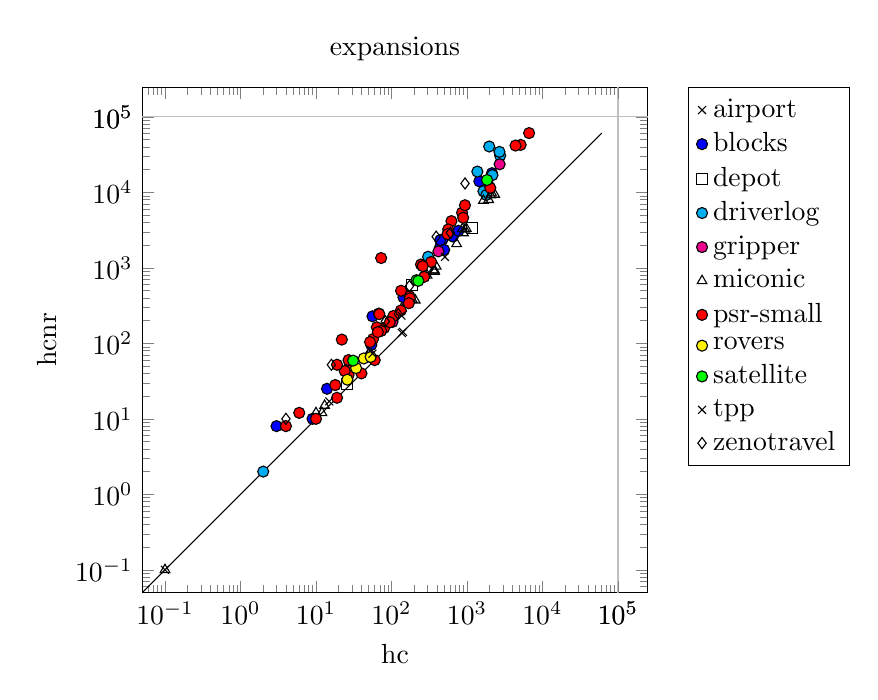
\begin{tikzpicture}
\begin{axis}[extra x tick style={grid=major}, extra x ticks=100000, extra y tick style={grid=major}, 
extra y ticks=100000, height=8.00cm, legend cell align=left, legend style={at={(1.4, 1)}}, title=expansions, width=8.00cm, xlabel=hc, xmin=0.05, xmode=log, ylabel=hcnr, ymin=0.05, ymode=log]
\addplot[color=red, mark=x, mark options={{draw=black}}, only marks] coordinates {
(0.100000, 0.100000) (137, 137) (142, 142)
};
\addlegendentry{airport}
\addplot[color=blue, mark=*, mark options={{draw=black}}, only marks] coordinates {
(100, 202) (1875, 13298) (2144, 17941) (439, 1855) (651, 2599) (3, 8) (14, 25) (499, 1732) (144, 407) (56, 228) (9, 10) (106, 219) (1458, 14012) (474, 2375) (70, 149) (54, 95) (770, 3093) (442, 2329)
};
\addlegendentry{blocks}
\addplot[color=cyan, mark=square, mark options={{draw=black}}, only marks] coordinates {
(1165, 3337) (26, 29) (186, 594)
};
\addlegendentry{depot}
\addplot[color=cyan, mark=*, mark options={{draw=black}}, only marks] coordinates {
(2176, 16918) (1652, 10340) (1805, 9221) (306, 1402) (1971, 40492) (2, 2) (2754, 30702) (1373, 18842) (2695, 34370)
};
\addlegendentry{driverlog}
\addplot[color=magenta, mark=*, mark options={{draw=black}}, only marks] coordinates {
(103, 192) (2708, 23542) (419, 1653)
};
\addlegendentry{gripper}
\addplot[color=blue, mark=triangle, mark options={{draw=black}}, only marks] coordinates {
(981, 3311) (1651, 7795) (188, 381) (2121, 9781) (12, 12) (371, 930) (730, 2078) (52, 77) (372, 890) (1940, 7993) (48, 63) (359, 929) (10, 12) (937, 3229) (51, 66) (164, 345) (0.100000, 0.100000) (47, 66) (46, 62) (13, 15) (2333, 9377) (296, 797) (391, 1046) (136, 290) (207, 372) (901, 2892) (2060, 9235) (867, 3283) (164, 351)
};
\addlegendentry{miconic}
\addplot[color=red, mark=*, mark options={{draw=black}}, only marks] coordinates {
(271, 760) (19, 19) (4, 8) (28, 55) (106, 230) (22, 112) (173, 421) (246, 1106) (27, 38) (5143, 42522) (68, 248) (27, 60) (861, 5382) (891, 4609) (60, 60) (80, 160) (64, 163) (6652, 60966) (24, 43) (57, 114) (73, 1348) (175, 395) (69, 244) (623, 4157) (18, 28) (52, 104) (73, 146) (6, 12) (2036, 11460) (95, 190) (134, 497) (564, 3227) (133, 272) (10, 10) (552, 2794) (335, 1194) (66, 141) (40, 40) (259, 1053) (941, 6750) (4401, 41680) (19, 52) (170, 340)
};
\addlegendentry{psr-small}
\addplot[color=yellow, mark=*, mark options={{draw=black}}, only marks] coordinates {
(34, 47) (43, 63) (53, 66) (26, 33)
};
\addlegendentry{rovers}
\addplot[color=green, mark=*, mark options={{draw=black}}, only marks] coordinates {
(214, 686) (227, 673) (1844, 14576) (31, 59)
};
\addlegendentry{satellite}
\addplot[color=green, mark=x, mark options={{draw=black}}, only marks] coordinates {
(56, 73) (136, 233) (511, 1394) (15, 17)
};
\addlegendentry{tpp}
\addplot[color=black, mark=diamond, mark options={{draw=black}}, only marks] coordinates {
(942, 13116) (123, 244) (4, 10) (173, 573) (16, 52) (602, 2919) (391, 2589) (83, 195)
};
\addlegendentry{zenotravel}
\addplot[color=black] coordinates {(0.050000, 0.050000) (60966, 60966)};
\end{axis}
\end{tikzpicture}
\\
        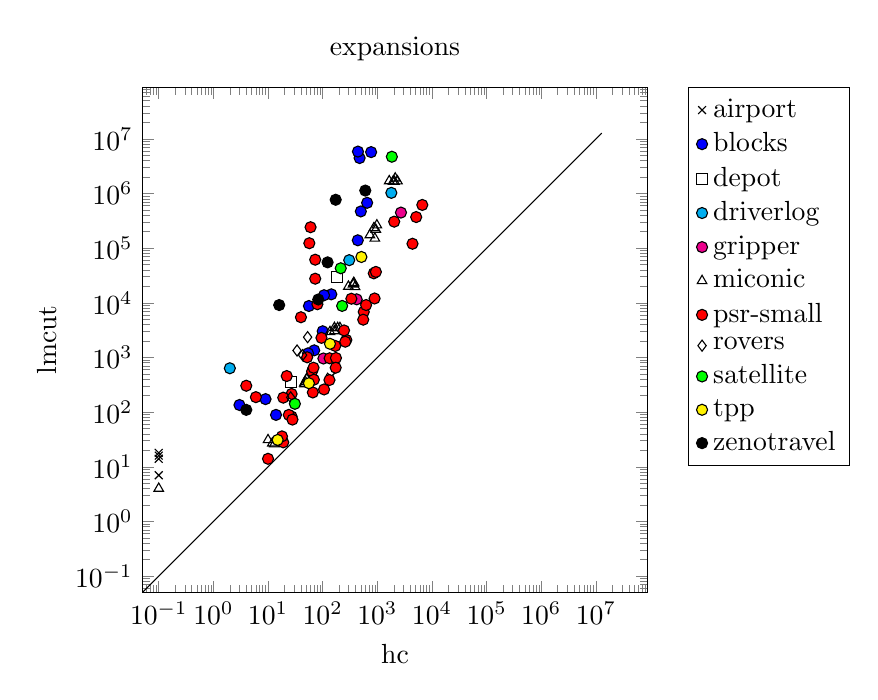
\begin{tikzpicture}
\begin{axis}[extra x tick style={grid=major}, extra x ticks=100000000, extra y tick style={grid=major}, extra y ticks=100000000, height=8.00cm, 
legend cell align=left, legend style={at={(1.4, 1)}}, title=expansions, width=8.00cm, xlabel=hc, xmin=0.05, xmode=log, ylabel=lmcut, ymin=0.05, ymode=log]
\addplot[color=red, mark=x, mark options={{draw=black}}, only marks] coordinates {
(142, 444) (0.100000, 14) (0.100000, 18) (0.100000, 7) (0.100000, 16) (137, 421)
};
\addlegendentry{airport}
\addplot[color=blue, mark=*, mark options={{draw=black}}, only marks] coordinates {
(9, 173) (474, 4460545) (100, 3018) (439, 139356) (14, 89) (144, 14312) (442, 5854588) (106, 13778) (56, 8750) (651, 676067) (770, 5723779) (3, 135) (70, 1350) (54, 1191) (499, 470462)
};
\addlegendentry{blocks}
\addplot[color=cyan, mark=square, mark options={{draw=black}}, only marks] coordinates {
(186, 30045) (26, 362)
};
\addlegendentry{depot}
\addplot[color=cyan, mark=*, mark options={{draw=black}}, only marks] coordinates {
(306, 60344) (1805, 1028572) (2, 635)
};
\addlegendentry{driverlog}
\addplot[color=magenta, mark=*, mark options={{draw=black}}, only marks] coordinates {
(103, 958) (419, 11586) (2708, 448198)
};
\addlegendentry{gripper}
\addplot[color=blue, mark=triangle, mark options={{draw=black}}, only marks] coordinates {
(2121, 1903853) (372, 22499) (48, 361) (13, 26) (52, 424) (391, 19586) (1940, 1650838) (12, 27) (730, 174147) (1651, 1697048) (51, 400) (2333, 1690274) (47, 327) (901, 151003) (359, 21853) (10, 31) (188, 3492) (46, 336) (371, 23396) (981, 263639) (207, 3488) (296, 19955) (0.100000, 4) (164, 3060) (867, 234915) (136, 2947) (937, 219412) (164, 3501) (2060, 1656771)
};
\addlegendentry{miconic}
\addplot[color=red, mark=*, mark options={{draw=black}}, only marks] coordinates {
(271, 2092) (27, 215) (861, 34633) (64, 557) (27, 83) (40, 5446) (80, 9432) (564, 6833) (73, 27640) (73, 61548) (6652, 618078) (259, 1944) (106, 260) (4401, 120468) (4, 304) (24, 89) (10, 14) (19, 28) (52, 1008) (623, 9112) (28, 73) (57, 123268) (95, 2286) (891, 12005) (552, 4917) (22, 457) (134, 967) (69, 392) (133, 387) (68, 649) (60, 241899) (335, 11892) (6, 188) (5143, 370920) (18, 36) (19, 184) (170, 1626) (175, 979) (66, 229) (941, 36799) (173, 650) (246, 3125) (2036, 305520)
};
\addlegendentry{psr-small}
\addplot[color=green, mark=diamond, mark options={{draw=black}}, only marks] coordinates {
(34, 1343) (43, 1106) (53, 2354) (26, 186)
};
\addlegendentry{rovers}
\addplot[color=green, mark=*, mark options={{draw=black}}, only marks] coordinates {
(214, 42892) (31, 142) (227, 8777) (1844, 4711577)
};
\addlegendentry{satellite}
\addplot[color=yellow, mark=*, mark options={{draw=black}}, only marks] coordinates {
(511, 69014) (136, 1779) (15, 31) (56, 338)
};
\addlegendentry{tpp}
\addplot[color=black, mark=*, mark options={{draw=black}}, only marks] coordinates {
(602, 1133103) (16, 9104) (4, 110) (123, 55014) (83, 11510) (173, 769022)
};
\addlegendentry{zenotravel}
\addplot[color=black] coordinates {(0.050000, 0.050000) (12763448, 12763448)};
\end{axis}
\end{tikzpicture}
\\
        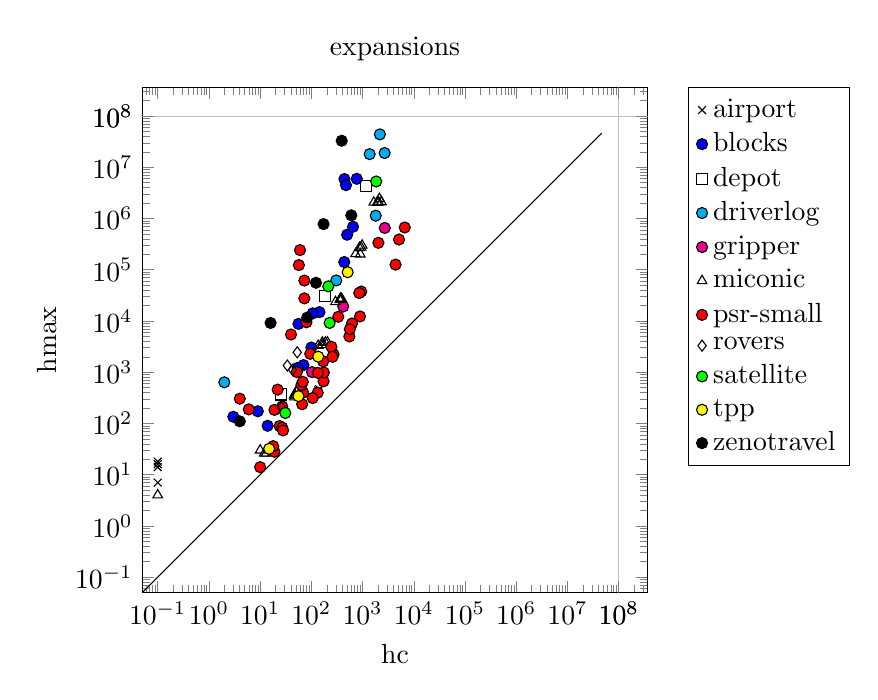
\begin{tikzpicture}
\begin{axis}[extra x tick style={grid=major}, extra x ticks=100000000, extra y tick style={grid=major}, extra y ticks=100000000, height=8.00cm,
 legend cell align=left, legend style={at={(1.4, 1)}}, title=expansions, width=8.00cm, xlabel=hc, xmin=0.05, xmode=log, ylabel=hmax, ymin=0.05, ymode=log]
\addplot[color=red, mark=x, mark options={{draw=black}}, only marks] coordinates {
(142, 464) (0.100000, 14) (0.100000, 18) (0.100000, 7) (0.100000, 16) (137, 441)
};
\addlegendentry{airport}
\addplot[color=blue, mark=*, mark options={{draw=black}}, only marks] coordinates {
(144, 14897) (9, 173) (442, 5894179) (70, 1376) (499, 483086) (56, 8783) (439, 141443) (100, 3031) (14, 90) (3, 135) (474, 4487213) (54, 1215) (651, 691186) (106, 14089) (770, 5968890)
};
\addlegendentry{blocks}
\addplot[color=cyan, mark=square, mark options={{draw=black}}, only marks] coordinates {
(186, 30239) (1165, 4348281) (26, 368)
};
\addlegendentry{depot}
\addplot[color=cyan, mark=*, mark options={{draw=black}}, only marks] coordinates {
(306, 61958) (1373, 18078718) (2695, 19007847) (1805, 1136659) (2, 635) (2176, 43967863)
};
\addlegendentry{driverlog}
\addplot[color=magenta, mark=*, mark options={{draw=black}}, only marks] coordinates {
(419, 19191) (103, 1006) (2708, 655342)
};
\addlegendentry{gripper}
\addplot[color=blue, mark=triangle, mark options={{draw=black}}, only marks] coordinates {
(51, 424) (372, 27235) (207, 3838) (13, 26) (1940, 2054791) (2333, 2104717) (48, 359) (10, 30) (188, 3838) (164, 3428) (46, 353) (47, 327) (730, 203857) (0.100000, 4) (981, 299347) (901, 201439) (937, 273423) (867, 269792) (136, 3311) (391, 27181) (371, 27525) (1651, 2066634) (296, 23696) (2121, 2441914) (2060, 2086171) (12, 26) (164, 3838) (52, 422) (359, 25847)
};
\addlegendentry{miconic}
\addplot[color=red, mark=*, mark options={{draw=black}}, only marks] coordinates {
(27, 215) (552, 4995) (133, 397) (335, 12092) (66, 237) (623, 8950) (40, 5446) (80, 9432) (73, 27640) (73, 61548) (271, 2230) (69, 400) (106, 313) (4, 304) (24, 89) (5143, 389358) (10, 14) (52, 1008) (19, 28) (57, 123268) (173, 665) (95, 2286) (891, 12261) (4401, 126004) (27, 83) (64, 561) (22, 457) (564, 6921) (6652, 668998) (175, 987) (68, 649) (60, 241899) (246, 3131) (6, 188) (134, 970) (28, 73) (18, 36) (2036, 335904) (19, 184) (170, 1626) (259, 2000) (941, 37611) (861, 35149)
};
\addlegendentry{psr-small}
\addplot[color=green, mark=diamond, mark options={{draw=black}}, only marks] coordinates {
(26, 207) (34, 1350) (53, 2442) (43, 1113)
};
\addlegendentry{rovers}
\addplot[color=green, mark=*, mark options={{draw=black}}, only marks] coordinates {
(227, 9176) (214, 47435) (1844, 5287951) (31, 160)
};
\addlegendentry{satellite}
\addplot[color=yellow, mark=*, mark options={{draw=black}}, only marks] coordinates {
(511, 89604) (56, 341) (15, 32) (136, 2013)
};
\addlegendentry{tpp}
\addplot[color=black, mark=*, mark options={{draw=black}}, only marks] coordinates {
(4, 110) (16, 9148) (123, 55748) (602, 1155505) (83, 11658) (391, 33028328) (173, 778708)
};
\addlegendentry{zenotravel}
\addplot[color=black] coordinates {(0.050000, 0.050000) (46590097, 46590097)};
\end{axis}
\end{tikzpicture}

    \end{center}
   